\documentclass[letterpaper, 12pt]{article}
\title{Gnuspeech ``Monet''}
\usepackage{wrapfig}
\usepackage{lipsum}
\usepackage{media9}
\usepackage{graphicx}
\usepackage{geometry}
\usepackage{hyperref}
\usepackage{amsmath}
\usepackage{amssymb}
\usepackage{MnSymbol}
\usepackage{afterpage}
\usepackage[justification=centering]{caption}
\usepackage{xcolor}
\usepackage{natbib}
\usepackage{longtable}
\usepackage{caption}
\usepackage{subcaption}
\usepackage{url}

\def\bsq#1{%both single quotes
\lq{#1}\rq}

\newlength{\myMheight}
\settoheight{\myMheight}{12pt}
\usepackage{tipa}
\newcommand{\ipauh}{\textschwa}
\newcommand{\ipaa}{\textturnv}
\newcommand{\ipae}{\textepsilon}
\newcommand{\ipai}{\textiota}
\newcommand{\ipao}{\textopeno}
\newcommand{\ipau}{\textcloseomega}
\newcommand{\ipaaa}{\ae}
\newcommand{\ipaee}{i}
\newcommand{\ipaer}{\textschwa :}
\newcommand{\ipaar}{\textscripta}
\newcommand{\ipaaw}{\textopeno :}
\newcommand{\ipaei}{\textepsilon\textiota}
\newcommand{\ipauhuu}{\textturnv\textcloseomega}
\newcommand{\ipaahuu}{\ae\textcloseomega}
\newcommand{\ipaoi}{o\textiota}
\newcommand{\ipaahi}{\ae\textiota}
\newcommand{\ipaw}{w}
\newcommand{\ipay}{j}
\newcommand{\ipar}{r}
\newcommand{\ipal}{l}
\newcommand{\ipap}{p}
\newcommand{\ipat}{t}
\newcommand{\ipak}{k}
\newcommand{\ipab}{b}
\newcommand{\ipad}{d}
\newcommand{\ipag}{g}
\newcommand{\ipam}{m}
\newcommand{\ipan}{n}
\newcommand{\ipang}{\textipa{N}}
\newcommand{\ipas}{s}
\newcommand{\ipaf}{f}
\newcommand{\ipath}{\textipa{T}}
\newcommand{\ipash}{\textesh}
\newcommand{\ipauu}{u}
\newcommand{\ipaz}{z}
\newcommand{\ipazh}{\textipa{Z}}
\newcommand{\ipav}{v}
\newcommand{\ipadh}{\textipa{D}}
\newcommand{\ipach}{\textteshlig}
\newcommand{\ipaj}{\textdyoghlig}
\newcommand{\ipah}{h}

\newcommand{\wbstuh}{\textschwa}
\newcommand{\wbsta}{\textprimstress\textschwa}
\newcommand{\wbste}{e}
\newcommand{\wbsti}{i}
\newcommand{\wbsto}{\textipa{\"a}}
\newcommand{\wbstu}{\.u}
\newcommand{\wbstaa}{a}
\newcommand{\wbstee}{\=e}
\newcommand{\wbster}{\oe}
\newcommand{\wbstar}{\.a}
\newcommand{\wbstaw}{\.o}
\newcommand{\wbstei}{\=a}
\newcommand{\wbstuhuu}{\=o}
\newcommand{\wbstahuu}{a\.u}
\newcommand{\wbstoi}{\.oi}
\newcommand{\wbstahi}{\=\i}
\newcommand{\wbstw}{w}
\newcommand{\wbsty}{y}
\newcommand{\wbstr}{r}
\newcommand{\wbstl}{l}
\newcommand{\wbstp}{p}
\newcommand{\wbstt}{t}
\newcommand{\wbstk}{k}
\newcommand{\wbstb}{b}
\newcommand{\wbstd}{d}
\newcommand{\wbstg}{g}
\newcommand{\wbstm}{m}
\newcommand{\wbstn}{n}
\newcommand{\wbstng}{\textipa{N}}
\newcommand{\wbsts}{s}
\newcommand{\wbstsh}{sh}
\newcommand{\wbstf}{f}
\newcommand{\wbstth}{th}
\newcommand{\wbstz}{z}
\newcommand{\wbstzh}{zh}
\newcommand{\wbstv}{v}
\newcommand{\wbstdh}{\underline{th}}
\newcommand{\wbstch}{ch}
\newcommand{\wbstj}{j}
\newcommand{\wbsth}{h}



\geometry{letterpaper,textwidth=16cm,textheight=24.5cm}

% End of preamble
%The body now follows

\begin{document}
\pagenumbering{roman}

\setlength{\topmargin}{-2.5cm}
\vspace*{4cm}
\begin{flushleft} {\LARGE \textbf{Gnuspeech TRAcT Manual 0.9}}\end{flushleft}
\noindent
\rule[6mm]{16cm}{1.5mm}
\vspace{-1.3cm}
\noindent
\begin{flushright} {\small{TRAcT: the Gnuspeech Tube Resonance Access Tool: a means of\\investigating and understanding the basic Gnuspeech vocal tract model}}\end{flushright}

\vspace{11cm}

\begin{flushleft} {\Large \textbf{David R. Hill, University of Calgary}}\end{flushleft}
\rule[7mm]{16cm}{0.9mm}

\vspace{-0.5cm}
\small{}TRAcT and the ``tube'' model to which it allows access was originally known as ``Synthesizer'' and developed by Leonard Manzara on the NeXT computer. The
name has been changed because ``Synthesiser'' might be taken to imply it synthesises speech, which it doesn't. It is a ``low-level'' sound synthesiser that models the human vocal tract, requiring the ``high-level'' synthesiser control inherent in Gnuspeech/Monet to speak. TRAcT provides direct interactive access to the human vocal tract model parameters and shapes as a means of exploring its sound generation capabilities, as needed for speech database creation.

\newpage

\vspace*{8cm}


\noindent{}(GnuSpeech TRAcT Manual Version 0.9)

\noindent{}David R. Hill, PEng, FBCS

\noindent{}(hilld@ucalgary.ca or drh@firethorne.com)

\noindent{}\textcopyright{} 2004, 2015 David R. Hill. All rights reserved.

\noindent{}This document is publicly available under the terms of a Free Software Foundation
``Free Documentation Licence''

\noindent{}See \href{http://www.gnu.org/copyleft/fdl.html}{see http://www.gnu.org/copyleft/fdl.html for the licence terms.}

\noindent{}This page and the acknowledgements section are the invariant sections.

\newpage

\begin{center}SUMMARY\end{center}

The ``Tube Resonance Model" (TRM, or ``tube", or ``waveguide", or transmission-line) forms the acoustic basis of the Gnupeech articulatory text-to-speech system and provides a linguistics research tool. It emulates the human vocal apparatus and allows ``postures'' to be imposed on vocal tract model, and energy to be injected representing voicing, whispering, sibilant noises and ``breathy'' noise. The ``Distinctive Region Model'' (DRM) control system that allows simple specification of the postures, and accessed by TRAcT \footnote{Other parameters representing non-postural variables such as temperature, tube length mouth and nose radiation characteristics are also provided}is based on research by CGM Fant and his colleagues at the Stockholm Royal Institute of Technology Speech Technology Laboratory (Fant \& Pauli 1974), by Ren\'e Carr\'e and his colleagues at T\'el\'ecom Paris (Carr\'e, Chennoukh \& Mrayati 1992), and further developed by our original research team at Trillium Sound Research and the U of Calgary). As noted

TRAcT forms part of the Gnuspeech text-to-speech system for serious speech research, for creating the databases for different languages, and provides a useful stand-alone demonstration and teaching tool, especially relevant to those wishing to use Gnuspeech.

If supplied with suitable parameter streams, the TRM is capable of producing synthetic speech, as is done in the complete articulatory speech synthesis system and language development application ``Monet'', or the kernel facility ``TextToSpeech
Server'' that provides speech ``Service'' for the system and for other applications that may be developed---all of these being part of the Gnuspeech software suite.

TRAcT is an essential tool in using ``Monet'' to build the databases needed to synthesise different languages, since it allows the required TRM configurations (the ``speech postures'') that are associated with the articulation of a language to be defined in terms of the control parameters for the TRM. Displays of the various TRM
quantities and controls are provided as components of the TRAcT GUI
interface

\newpage
\tableofcontents
\newpage

\section{Introduction}
\pagenumbering{arabic}

\subsection{Purpose of the system}

TRAcT allows speech researchers to understand the properties of
transmission-line analogues of the human vocal tract---the TRM in particular, and to assist in creating the posture databases for arbitrary language development, needed to drive the TRM within the context of the ``Gnuspeech'' articulatory speech synthesis system. The GnuSpeech system was originally developed to allow spoken language to be synthesised automatically by machines with greater fidelity and control than has previously been possible, based on a new articulatory vocal tract control model derived from work by Fant, Carr\'e and others, as summarised in (Hill, Manzara \& Schock 1995).

\subsection{Background}

Early history: Work on speech synthesis has been going on from early times. The advent of modern electronics and signal processing methods in the 40s and 50s led to a surge in progress. Targetted research, initially at Bell Labs and the Haskins Laboratories (then in New York), using the new Sound Spectrograph, together with other aids, began to unravel the acoustic cues for speech. Military research was also involved because achieving secure communication and voice transmission bandwidth compression, both depended on better understanding of speech structure.

\begin{figure}[htb]
\centering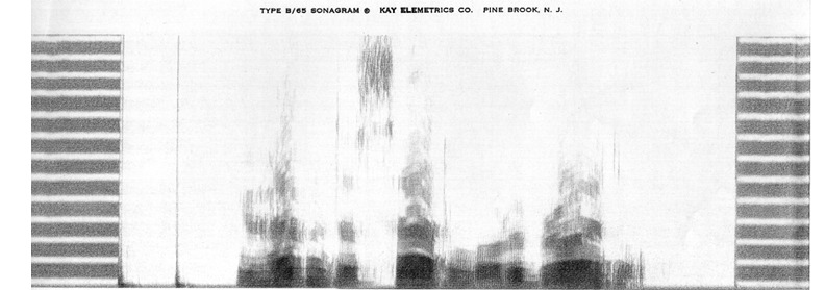
\includegraphics{images/shadfax5pd}
\caption[Spectrogram]{\label{shad-fax}Spectrogram of the author reading JRR Tolkien's Lord of the
Rings:\\
``You haven't a saddle or a bridle'' referring to Gandalf on Shadowfax
(Tolkien 1966)\\(\textbf{Note:} the bands up either side at 500 Hz intervals, provided
for calibration purposes)}
\end{figure}

The Sound Spectrograph was invented at the Bell Laboratories and was built commercially by the Kay Electric Company (later the Kay Elemetrics Company) as the Kay ``Sonagraf''. The device used a scanning filter to produce an analogue presentation of the amount of energy at present different frequencies in a time varying input waveform. Spectrograms (``Sonagrams'') produced by this machine showed the variations in energy, as darkness of marking, against time and frequency-so-called ``visible speech'' (Potter, Kopp \& Green 1947) as in Figure 1. The most striking features seen in a speech spectrogram are varying dark bands, representing the moving spectral energy peaks created by vocal tract resonances as different postures follow one another (these resonances are called ``formants''); breaks in the energy due to stop sounds such as ``t'', ``d'' ``b'' (in this sample); and segments of noise.

When the device was first invented, it was thought that problems of speech recognition and speech input for the deaf were solved, but it took two years of full-time training to allow people to ``read'' visible speech, and not all people were successful, and machines were unable to use the cues as effectively as people did. One of the difficulties is knowing where words begin and end. We hear them quite distinctly, but acoustically there are, in general, no consistently clear boundaries, as may be seen in Figure \ref{shad-fax}. The machine was later redesigned using digital technology, replacing the scanning filter with a real-time Discrete Fourier Transform (DFT) analysis algorithm (a digital equivalent of the Fourier Transform that works on discrete time samples of the waveform rather than an analogue waveform). This approach avoided the many problems of calibration and adjustment that plagued the earlier machine, whilst producing equivalent results. More recently readily available computer software has been developed, the most notable system being ``Praat" (Boersma 2001; Lieshout 2003). The various displays/analyses that can be produced are outstanding.

The first successful parametric speech synthesiser---Lawrence's ``Parametric Artificial Talker'' (PAT) (Lawrence 1953; 1954) toured the US in the mid-1950s. It was based on simulating the formant structure of speech by means of cascaded filters, and required compensation for the output impedance of the mouth, higher formants, as well as a source of glottal excitation and noises. The nasal cavity was absent whilst frication and aspiration were approximated by random noise generation and filtering (through the vocal tract filters in the case of aspiration). The data needed to produce synthetic speech (by varying the formant frequencies and other parameters) was initially copied from spectrograms of real speech.

As knowledge grew, Pierre Delattre at Haskins came to understand enough to generate synthetic speech from the Haskins Pattern Playback (PB) machine without reference to any particular real utterance. PB used a spinning wheel to produce a set of frequencies by modulating light  passing through the wheel, and ingeniously recreated speech from painted spectrograms, using either the reflected light or the transmitted light, rather than using a limited set of formant filters. The difference from PAT is somewhat akin to pixel images (spectrogram) versus vector graphics (parametric descriptions) but, unlike PAT and similar machines, the speech was monotone.

Soon rules for producing appropriate parameter variations for formant synthesisers like PAT were developed, mainly based on the Haskins work, and synthetic speech was truly on its way.

Experiments with electrical transmission-line models of the vocal tract began around this time in several laboratories. A transmission-line, waveguide, lattice filter, or tube model all are terms to describe the same technique which simulates (emulates) the acoustic properties of a physical tube with air in it -a tube having a high impedance source one end, and a variable opening the other, plus the ability to vary the cross-sectional area along the length. The first such device, a 25 T-section circuit incorporating both oro-pharyngeal and nasal tubes, was built by Dunn (1950) at the Bell Telephone Laboratories.

Hecker (1962) Describes addition of DANA, the Dynamic nasal passages analogue, to DAVO, the Dynamic vocal tract analogue at the MIT Research Laboratory of Electronics (RLE). Stevens et al. (1953) describe further work at the RLE.

Gunnar Fant, in his classic seminal work ``Acoustic Theory of Speech Production'' (Fant 1960)-a book based on his doctoral thesis which was examined in front of the King of Sweden by a panel of examiners that included Walter Lawrence-discusses T-section transmission-line analogues of the vocal tract (Fant 1960, p 26 et seq.). Fant opens the relevant section as follows:

\begin{quote}\footnotesize ``The mathematical treatment of the speech production process involves the following successive operations. The first one is the mapping of the vocal cavities in terms of an area function describing the cross-sectional area perpendicular to the air stream from the glottis to the radiating surface at the lips. Secondly, this area function has to be approximated by a sufficiently small number of successive parts, each of a constant cross-sectional area. The transmission properties of this system are next calculated and added to the assumed characteristics of the source. The last step is to perform a maximally concise presentation of the results by converting the calculated frequency characteristic into a set of poles and zeros  [resonances and anti-resonances]. When dealing with voiced sounds  [sounds in which the vocal folds within the glottis are vibrating] the formant frequencies are of primary interest.'' \normalsize\end{quote}

Implementing ``\textellipsis a sufficiently small number of successive parts, each of constant cross-sectional area.'' (i.e.~the need for a not-too-numerous set of concatenated cylindrical tube section equivalents) proved to be a significant problem for these electrical analogues. Although Dunn's device had only twenty-five sections to represent both oro-pharyngeal and nasal cavities and the radiation impedance at nose and lips, it was generally considered that around forty sections were required just for the oro-pharyngeal cavities to achieve a reasonably smooth approximation. Collecting and using the amounts of data needed for such detailed control constituted two serious problems, which have only been partly addressed in their pure form up to the present time. In addition, the electrical circuits of those days were plagued by problems of instability and calibration-problems that have largely been solved by the advent of digital approaches to modelling.

Many labs were active in speech research in those days, too many to list. Some were commercial, many were at universities around the world. Military establishments were also active because a parametric analysis and re-synthesis of speech gave promise of secure voice communications by scrambling the parameters in some way, as a form of encryption. This was the basis of the scrambler telephones of the Second World War, but the technology was closely allied to the requirements of speech recognition and synthesis. The conversion of speech into a small number of slowly varying parameters was also of interest for purposes of transmission bandwidth reduction. The parameterisation process effectively jettisoned all the information except that needed to understand the words-at least in theory. As a result, the number of bits required per second of speech was reduced from around 30,000 for telephone speech to perhaps less than 4,000 for parametric speech. This was important in the days of limited bandwidth on channels such as submarine cables. Times were exciting, and progress dramatic, though often far short of goals.

``Speech Synthesis''-the book edited by Flanagan (1973)-provides a collection of papers that cover this early history quite well (though Lawrence's seminal contribution is inexplicably omitted, apart from a couple of citations within included papers).
 
The formant synthesiser was also called a ``source-filter'' model, because the excitation energy (glottal vibrations or noise or both-the source) was filtered through the formant filters. A major problem for analysis-synthesis telephony was that of determining the pitch of glottal excitation, a problem which is still not completely solved. Another problem with the glottal source is that it controls the intonation of an utterance according to rules which are still relatively ill-understood. The intonation can affect the meaning of an utterance quite drastically, even reversing the meaning. Rhythm creates similar problems for much the same kind of reason. Consider the reply to an agreement to meet at (say) 3pm. The respondent can say: ``No, earlier'' (we mustn't meet later than 3) or ``No earlier'' (we mustn't make it before 3). The difference is one of intonation and rhythm which, together, constitute prosody.

More recently, speech has been synthesised by concatenating small segments of real speech together. It is not clear that concatenating recordings of larger portions of real speech counts as synthesis, though useful systems have been produced that build up utterances on this basis. In either case the problems of rhythm and intonation have to be solved. The original intonation is usually removed these days by using Linear Predictive Analysis of the waveform, in which the value of the next digital sample in the time series representing the digitised speech waveform is predicted as a linear function of past values. This allows the source and filter components to be separated, as required. The early work in this area is best accessed through two seminal works: a paper by Atal and Hanauer (1971) and a book by Markel and Gray (1976). There are sheep and goats when it comes to speaking, and the recordings made by sheep are the easily analysable ones. They are also the ones that are used to show off the performance of speech recognisers-but that is another story. Separation of source and filter components can also be achieved using Cepstral analysis.

Carefully done, with precautions to deal with the joins between segments, excellent speech quality is possible, in terms of natural voice quality, using concatenative methods. With restricted speech, precomputed intonation and rhythm may be imposed by recombining the source and filter components by an inverse process, but difficulties remain. For example, extending the vocabulary, changing the ``speaker identity'', and dealing with imperfections all raise problems that are only partly solved.

\subsubsection{Background to ``TRAcT''}
\label{smith}

Fant and Pauli (1974) went on to perform a sensitivity analysis for the effect of constrictions in the vocal tract on formant frequency. The work showed that the changes in formant frequency could be described fairly simply, and were related to where the constriction was in relation to the nodes and anti-nodes of the formant resonances within the acoustic tube. Apart from the original work just cited, a simple explanation of the underlying theory is provided in Hill et al. (1995). Suffice it to say here that Formant 1 (the lowest resonance) is raised in frequency by a constriction in the first half of the tube beginning at the glottis, and lowered by a constriction in the second half that terminates at the lips. Formant 2 divides the tract into four regions-raises, lowers, raises, lowers. Formant 3 divides the tract into six regions with similar alternation of raising and lowering its frequency. When combined, these various regions produce eight distinct regions of the vocal tract in which the combinations of raising and lowering the three formants are co-determined-it can, in fact, be considered a kind of binary encoding of the eight regions in terms of raising/lowering each of the three formants, as shown in Figure \ref{drm-const}.

\begin{figure}[htb]
\centering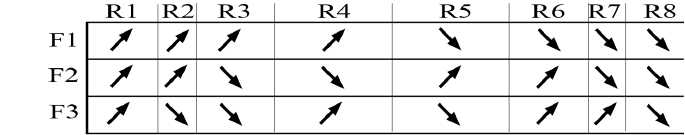
\includegraphics{images/effect-of-constriction-_opt}
\caption[Effect of DRM constrictions]{\label{drm-const}The effect of constrictions in DRM regions R1 to R8}
\end{figure}

The regions differ in length and, for a given formant, the amount of raising or lowering of the frequency depends on the exact placement within the underlying sensitivity region. Thus, for example, constricting the tube at the lips (i.e.~in the R8 region) has a greater lowering effect on the formant 1 frequency than a similar constriction nearer the node for that formant-in the R5 region. It should also be noted that, according to the theory, when cross-sectional areas of intermediate constrictions are set lower than about 1cm2, the conditions for the DRM model are no longer met and the tube begins to approach a two or three tube model, rather than a constricted single tube. But that is true of the real vocal tract too.

It is important to know that just the three lowest formant frequencies are necessary and sufficient for establishing the identity of all formant-based speech sounds. Higher formants exist, and add to both the naturalness and intelligibility of the speech, but they do not distinguish between different phonemes2 by any independent variation.

Carr\'e and his colleagues took Fant and Pauli's work and proposed a method of vocal tube control which they called the Distinctive Region Model (DRM). The vocal tract was considered to comprise eight cylindrical regions corresponding to the regions distinguished by their effect on raising/lowering formant frequencies. The question as to how much this simplification affects the resonant behaviour has not been examined but, in general, introducing discontinuities into a transmission line produces reflections. How sharp discontinuities (as in the DRM) differ from smoothed discontinuities (as in the real vocal tract) remains to be experimentally verified. One main theory that Carr\'e and his co-workers investigated at the time (early 1990s) was that vowel-consonant-vowel utterances could be adequately modelled by superimposing a consonant closure on a vowel-to-vowel gesture using the DRM. They took real speech analyses and compared them with formant transitions obtained from the DRM model results obtained by the stated superposition, using specified transition shapes (e.g.~cosines). Among their conclusions: ``The DRM model is able to reproduce the \"O�hman (1966) V1-C-V2 trajectories with a very good accuracy.'' (Carr\'e \& Chennoukh 1993).

Their work highlighted the idea that an accurate model of articulation, related to the known properties of the real vocal tract and requiring only eight independently controlled sections, could be built and controlled dynamically, instead of requiring the forty or so that seem to be needed if the actual vocal tract properties are ignored. The topic is discussed more fully in the paper by Hill, Manzara \& Taube-Schock (1995) ``Real-time articulatory speech synthesis by rules''. The controlled sections correspond closely to the distribution of articulatory possibilities in the vocal tract (Carré et al. 1994) so that, even though the traditional parameters such as jaw rotation, tongue height, and so on are not used directly, the model does vary the tube shape and is truly an articulatory model. The traditional parameters could be used to define the changes in the DRM regions by using appropriate connecting equations. Provision for this intended extension has been made in the basic framework of the ``Monet'' system but is beyond the scope of the present manual.

\begin{figure}
\centering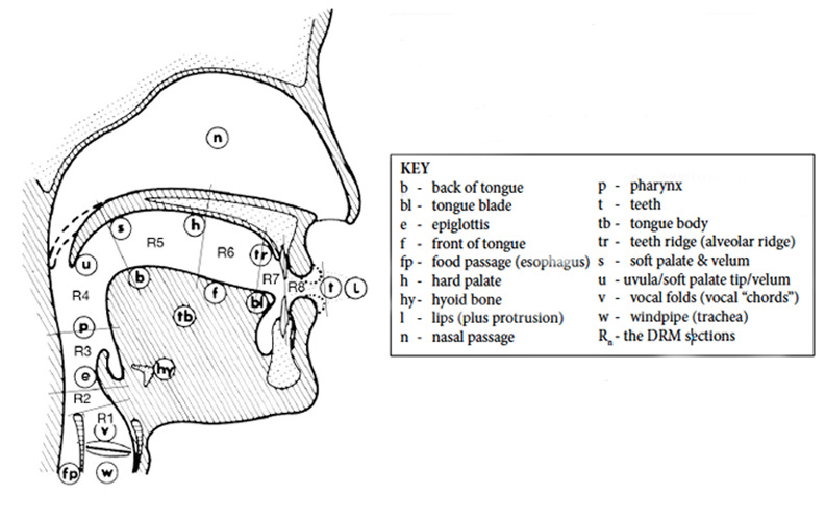
\includegraphics{images/saggital-w-key+cap}
\caption[DRM mapping onto vocal tract]{\label{drm-map}Mapping the DRM onto the human vocal apparatus}
\end{figure}

Waveguide models have been used for a variety of purposes, including the emulation of musical instruments. The work by Julius Smith, Perry Cook and their colleagues at the Stanford University Center for Computer Research in Music and Acoustics (CCRMA) was seminal, and included the availability of their ``Music Kit'' and waveguide software. Perry Cook developed SPASM an eight region articulatory model for singing for his thesis research under Julius Smith. The sections were of equal length, rather than sized to approximate the DRM (Cook 1991). His software was accessible to us during the development of our TRM, and was an important resource.

TRAcT and the Tube Resonance Model, the subjects of this manual, were developed as part of a commercial venture to create a new text-to-speech system based partly on the author's research, including rhythm and intonation, at the University of Calgary as well as earlier work. The whole project took about a year---mostly in 1994---and was conducted in an official university spin-off company we set up.

TRAcT was developed because hands-on access to the TRM was essential to creating the articulatory posture data needed as part of the text-to-speech database for the complete text-to-speech system. Such data simply did not exist. It also allowed the TRM to be examined and tested extensively to validate the tube implementation. A paper published on the web by Julius Smith provides an excellent, succinct resource for pretty well all aspects of the relevant topics, as well as a rich collection of links (Smith 2004). His characterisation of waveguide synthesis in that comprehensive work is illuminating:

\begin{quote}\footnotesize
``A (lossless) digital waveguide is a bidirectional delay line at some wave impedance R. \textellipsis since we now have a bidirectional delay line, we have two traveling waves, one to the `left' and one to the `right', say. It has been known since 1747  [74] that one-dimensional, linear, acoustic vibration can be described with complete generality as the sum of two traveling waves going in opposite directions. Thus, while a single delay line can model an acoustic plane wave, a bidirectional delay line (a digital waveguide) can model any one-dimensional linear acoustic system, such as a violin string, clarinet bore, flute pipe, trumpet-valve pipe, or the like. Of course, in real acoustic strings and bores, the 1-D waveguides exhibit some loss and dispersion  \textellipsis so that we will need some filtering in the waveguide to obtain an accurate physical model of such systems.''
\normalsize\end{quote}

A tube model of the vocal tract emulates rather than merely simulates the resonant behaviour of the vocal tract because the tube behaviour maps directly onto the articulatory and acoustic characteristics of the real vocal tract, nasal passage and radiation impedance of nose and mouth---it doesn't just imitate the resonance-mediated output using filters, as a formant-based synthesiser does. The current TRM is somewhat hybrid, as it stands, because the glottal waveform and frication/aspiration noises are created as waveforms and injected at appropriate places rather than being created by detailed fluid-mechanical models of the vibrating vocal folds and noise-making constrictions in the tract. In this sense, it is still a source-filter model, but the tube filter embodies all the important features of reality, including the energy balance between nasal and oro-pharyngeal cavities, the energy balance between radiated and reflected energy at the mouth and nose, the continuity constraints on the tube itself, and the production of accurate higher formants, so that the quality of the speech is potentially far higher than with contrived formant filter models or spectrogram playback approaches. It is the reflection at the mouth and nose that creates the travelling wave(s) in the opposite direction to what originates at the glottis.

The remainder of this manual will explain the functional aspects and use of the Tube Resonance Model, as implemented, through the TRAcT Application.

In dealing with the machine perception and production of speech, a number of technical terms must inevitably be used in order to achieve precision of expression.. The reader's attention is drawn particularly to the terms associated with speech sounds (phones, phonemes, postures, etc) and the basic concepts associated with rhythm and intonation. \href{http://pages.cpsc.ucalgary.ca/~hill/papers/conc/index.htm}{(Hill 1991)}, accessed 2015-05-06, provides a source of such conceptual knowledge, as noted.

\section{System overview and rationale}

\subsection{Introduction}

Figure \ref{all-win} shows a full screen view of the system in operation. The sound output is the ultimate validation of the configurations created for the tube model, in terms of data needed for speech synthesis, as verified by the spectral display. Figure \ref{anal} shows an ``Analysis'' panel whilst an ``ee''-like sound is being generated. There follows an extensive discussion of speech analysis techniques in the context of the Analysis subsystem. This is done to clear the decks for the rest of the overview, and provide the background needed for the section on using the system, because a good understanding of the Analysis subsystem theory is very helpful for interpreting the analyses of the sounds produced, and thereby judge the effectiveness and appropriateness of any configurations developed.

Note that in the various graph displays, the logarithmic scales are currently inactive.

\begin{figure}[htb]
\centering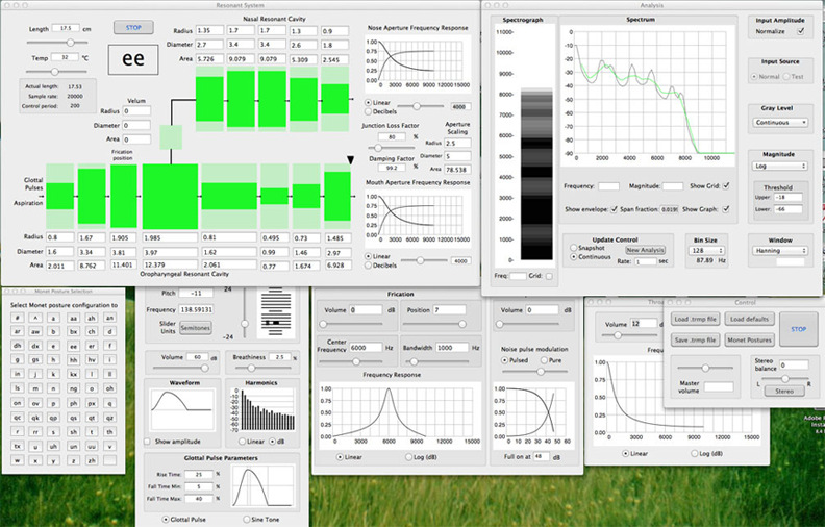
\includegraphics{images/all-windows-2}
\caption{\label{all-win}Full screen view of all the ``TRAcT'' windows}
\end{figure}

Figure \ref{all-win} shows all the TRAcT windows whilst running it is running. The ``Tools'' menu at the top of the Macintosh OS X screen (not visible in this view) gives access to the various panels that may be brought up to control the TRAcT facilities: (a) the main window-representing ``Resonant System'' itself with, provision to vary the tube regions by direct manipulation as well as other basic properties; (b) the ``Analysis'' system that allows spectra to be produced representing the frequency content of the tube output; (c) the ``Select Monet Posture'' panel that allows the tube configurations for the various existing ``Monet'' postures to be called up, examined and (where appropriate) heard; (d) the ``Glottal Source'' generator; (e) the ``Noise Source'' generator that controls both aspiration and frication noise, and allows pitch-pulse-timed modulation of the frication noise; (f) the control for the frequency characteristics of ``Throat Transmission'' (energy leaking through the tissues of the throat); and (g) the ``Control''panel which includes saving and restoring configurations that have been created, reloads the default values, and gives alternative access to both the ``Run/Stop'' toggle and the ``Select Monet Posture'' panel.

\subsubsection{The spectral analysis subsystem}

\begin{figure}
\centering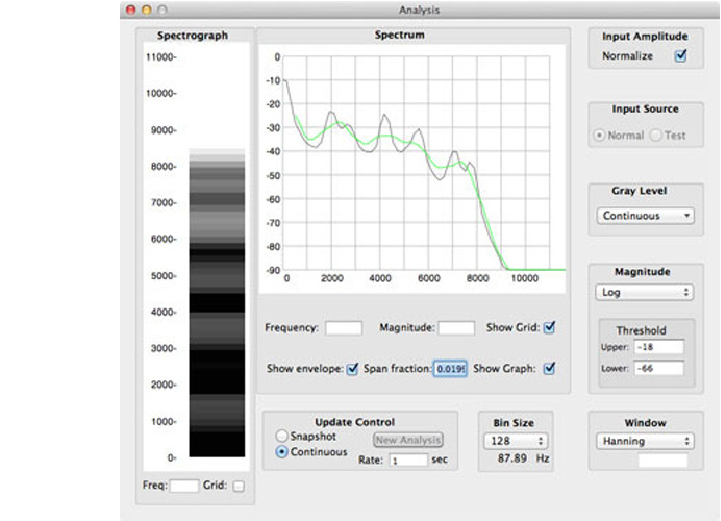
\includegraphics{images/analysis}
\caption{\label{anal}The analysis window}
\end{figure}

Figure \ref{anal} shows the Analysis window during production of an ``ee''-like sound (/i:/). The DFT has decomposed the digitally sampled time waveform into its underlying frequency components---an operation that is crucial to instrumental speech research. The human ear performs an equivalent analogue-to-digital frequency analysis of the input sound waves along the ``basilar membrane'', within the ``cochlea'' (part of the inner ear), and converts the output to digital form for further processing in the higher auditory pathways and auditory cortex. It has been found that the time structure of this information is more important than the frequency content (Whitfield \& Evans 1965), which has implications for understanding the structure of speech.

On the left of the panel is a window in which a spectrographic representation of the frequency content may be presented. This display does not show any time variation, but only the spectrum of the output signal, at the time it is sampled. A grid may be superimposed on the display, for convenience, by checking the box below the display. Also, moving the cursor on the spectrogram causes the frequency at the tip of the cursor to be displayed in the frequency box next to the check box. The spectrograph display is intended to allow the user to relate the output of the TRM to spectrograms of utterances produced by other means.

The main spectral display is in the middle of the panel and shows the TRAcT output spectrum which is a time cross-section of the spectrogram. The display allows the user to gain a better idea of the spectral shape of the individual formant peaks which may even be hard to separate in a spectrographic display. Boxes between the ``Spectrum'' display and the ``Update Control'' area show the frequency and magnitude (in decibels) for the cursor position within the spectrum window. There is also a check box to turn the grid on and off.In addition, two fields below the graph show the ``Frequency'' and ``Magnitude'' of the point where the cursor is positioned

There are a number of controls in the ``Update Control'' area. Two radio buttons allow the analysis to be performed either as a ``Snapshot'' or on a regular timed basis (``Continuous''). The interval between successive analyses in ``Continuous'' mode is determined by the value, in seconds, entered in the ``Rate'' box. In ``Snapshot'' mode, the ``Do Analysis'' button must be clicked.

The ``Bin Size'' box allows the number of samples for inclusion in the sampling window (see below) to be set. The frequency beneath the selector menu shows the equivalent bandwidth of the resulting filter effect. Window sizes from 16 to 512 samples may be chosen.

\subsubsection{Spectrograms and spectral sections}

It is necessary to say a little about spectral analysis. This section is illustrated using reproductions of Sonagrams produced by a Kay Sonagraf because the spectrograms produced by TRAcT are relatively simple and do not illustrate time variation, which disguises some important facts.

Figures 6a through 6d show the effect of different analysing bandwidths and frequency scalings on the resolution and appearance of speech spectrograms (the same reading as Figure \ref{shad-fax}. Figure 6a presents just the speech portion, Figure 6b is then a frequency expanded version of Figure 6a. Both have an effective analysing bandwidth of 300 Hz. This is a relatively wide bandwidth and brings out the envelope structure of the spectrum. In analysing a signal, there is a time/bandwidth trade-off. To observe the time structure, you need a fairly wide, fast response filter and the price paid is less frequency resolution. This is appropriate for speech formant analysis because the formants represent the peaks of the spectrum envelope while the fine time resolution allows the successive articulations to be seen and (as far as it is possible at all) the successive articulations to be separated. In practice, the boundaries between successive articulations (which are instantiations of phonemes, i.e. ``phones'') are only placed as a result of judgement, based on experience coupled with somewhat inconsistent rules of phonetic analysis. In addition, the fine time resolution allows the damped resonance oscillations invoked by each pitch pulse to be seen as vertical striations running vertically across all resonant frequencies carrying voiced energy rather than noise excitation. Pitch synchronous analysis is one way of solving the ``cocktail party'' problem, in which different speaking sources must be separated. It is also a powerful approach to instrumental analysis.

\begin{figure}[htb]
\centering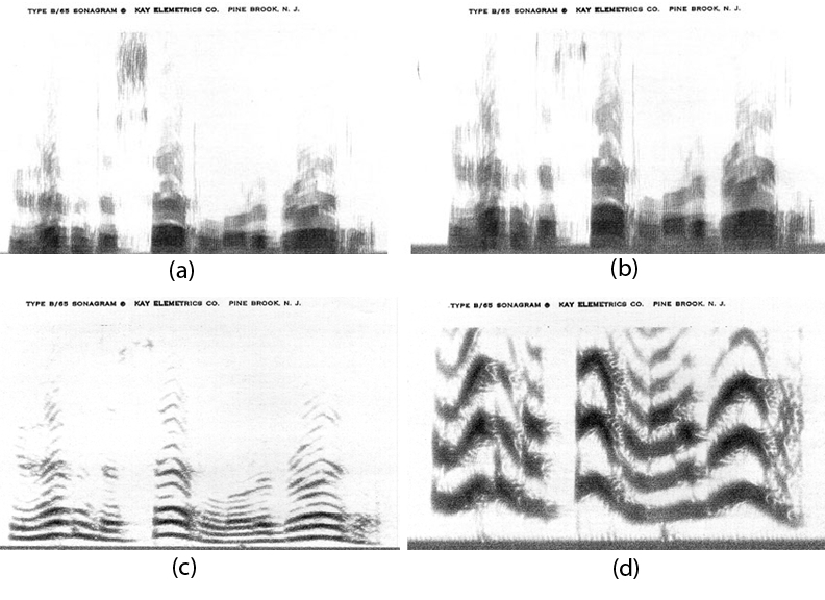
\includegraphics{images/fig-6}
\caption{\label{spect-w-n}Wide and narrow spectrograms with different ranges}
\end{figure}

\vspace{12pt}

Figures 6c and 6d show the same portion of speech analysed with a narrow filter bandwidth that is effectively 150 Hz. Figure 6d is a frequency expanded version of 6c that only goes to 850 Hz rather than 6000 Hz or 4200 Hz (frequency is on the y-axis, time on the x-axis). In both cases, because the analysing filter has great frequency resolution and less time resolution, much of the fine time structure is lost. The dominant features of the spectrograms are the pitch harmonics which vary more slowly than the features associated with articulation. The glottal waveform is (to a crude first approximation) a triangular waveform, so a complete harmonic spectrum at multiples of the pitch frequency is produced. The greatly expanded spectrogram of Figure 6d is used to get accurate manual tracings of the variation in pitch frequency in order to conduct research on intonation patterns. This is the reason these particular spectrograms were produced in the first place. The broad band analyses allow a ``segmental analysis'' (a determination of the successive speech sounds---phones, the instantiations of English phonemes, as previously noted), and the narrow band analyses allow the quantitative variation in pitch to be accurately correlated with these segments.

\subsubsection{Analysis sub-system spectral analysis options}

Similar options for analysis are included in TRAcT to allow comparison with analyses produced from other systems and also because they are familiar to speech researchers.

\begin{figure}[htb]
\centering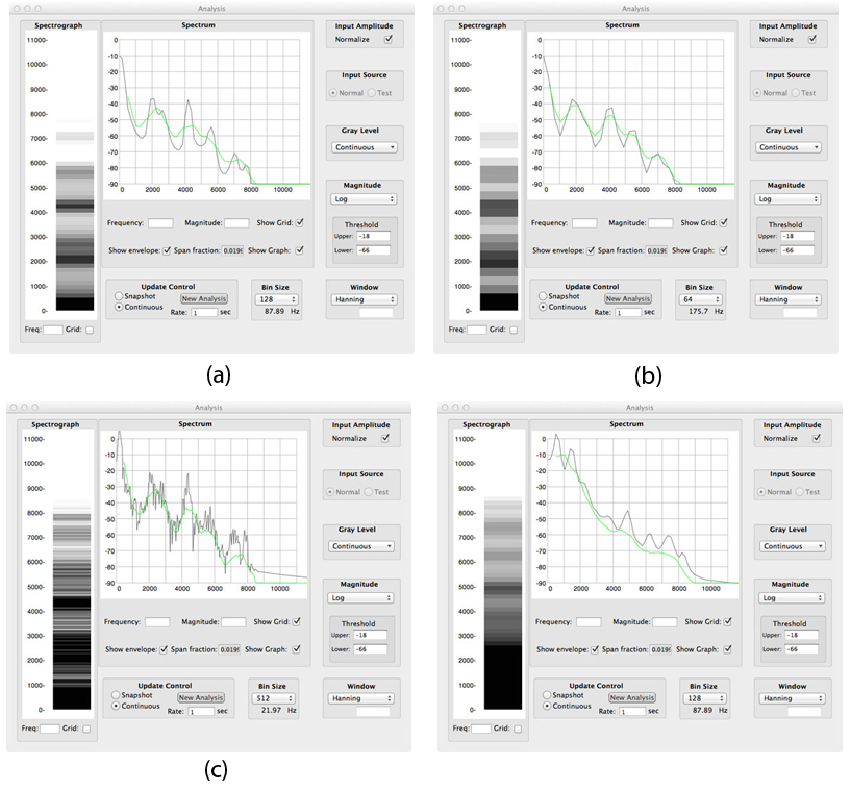
\includegraphics{images/fig-7}
\caption{\label{trac-w-n}TRAcT wide and narrow band spectrograms}
\end{figure}

At present, steady-state sounds (or one-at-a-time snapshots of a varying TRM output) can be analysed. With current hardware and some work, the system could be adapted to a more comprehensive spectrographic analysis of the speech output from the complete GnuSpeech system (i.e. continuous synthetic speech), and the quality of all the displays improved. However, the Praat system (Boersma 2001; van Lieshout 2003) renders such an exercise redundant.

Since the Analysis sub-system stores the output samples from the TRM to be used for analysis in an array bigger than is used for the largest sampling window, a sound can be subjected to more than one analysis by changing the settings.

Figures 7a and 7b show two analyses for an ``ee-like'' sound using the TRAcT ``Analysis'' tool. Figure 7a is a typical wide-band analysis of a sound like English ``ee'' with displays using a 128-point-pcm-sample (128 point ``Bin size'') and a Hanning window. Other sampling window shapes are available (see below section 2.2.6). The presence of low formant 1 and high formants 2 and 3, characteristic of this sound, is obvious in the spectral (time-cross-section) display. Formants 4 and 5 are higher still. The remaining formants do not show on the display as they are below the display threshold The green plot is an smoothed envelope for each plot. It, and the grid lines and graph can all be turned off separately.

Figure 7b is a similar analysis done with a sample window size (``Bin Size'') of only 64. With the wider band analysis, it is more difficult to separate the formant peaks, or get an idea of their exact frequency, or even the shape of the spectral section. 

Figure 7c is again an ``ee'' (/i/) sound, but this time done]with a window size of 512. In this display the individual pitch]harmonics are clearly visible in both the spectral section display and]the spectrum. Again it is less easy to pick out the value of the formant]peaks from the basic plot.

Figure 7d provides the output for an ``aa'' sound (/\ipaaa/) sound using 128 signal points and a Hanning window for comparison. The crude envelope is much less helpful here. 

Wells (1963) found frequencies of 285, 2373 and 3088 for the first three formants of the vowel sound /i/ in the word ``heed'', for 25 speakers with a British English ``Received Pronunciation'' (RP) accent. He examined ten such vowels altogether (/\ipaee, \ipai, \ipae, \ipaaa, \ipaar, \ipao, \ipaaw, \ipau, \ipauu, \ipaa, \ipaer/. We used the formant frequency values determined as a guide in setting up the nominal Gnuspeech vowel formant values, and our results may be examined by choosing the ``Open Monet Posture" tool from the ``Tools'' menu in TRAcT.

\subsubsection{Cepstral analysis and smoothing}

A useful facility that is not provided for the Analysis panel Spectrum display, but should be in the future, is a more sophisticated spectral smoothing function to allow the narrow-band analyses to be processed into a smoothed form that would show the peaks more clearly. There is a whole field of study related to this requirement associated with Cepstral techniques and LPC analysis (see above). In Cepstral analysis, the envelope of the initial spectrum produced from the original time-domain waveform can itself be treated as a ``pseudo-time-domain waveform'', and subjected to further ``spectral'' analysis, producing a ``Cepstrum''. The Cepstrum is in the so-called ``Quefrency'' domain, just as the Spectrum is in the Frequency domain. The high quefrency components in the cepstrum (resulting from the pitch harmonics in the original spectrum) can be removed, and an inverse DFT applied. The result is a smoothed spectrum, with a separate measure of the pitch frequency. Further discussion of this topic is outside the scope of the present manual. Check it out on the web. A quick summary appears in the author's Conceptionary for speech and hearing (Hill 1991).

\subsubsection{Additional analysis controls}

There are additional controls on the right-hand side of the Analysis panel. The ``Input Amplitude Normalize'' check box, when checked, allows arbitrary input waveforms to be normalised to the best range for analysis. The Gray Level can choose ``Continuous'' shading or ``Quantised'' shading for the Spectrograph display. Below that is a menu to choose ``Log'' (logarithmic) or ``Linear'' scaling for the Spectrograph and Spectrum displays. The ``Input Amplitude Normalize'', ``Gray Level'' and Magnitude selections are currently inactive. The ``Threshold'' fields below those allow the levels to be set for the spectrograph shading. The ``Upper'' value determines the completely black level. All energy levels at that level and above will display as the blackest shade. The ``Lower'' value determines the level at and below which the shading will be completely white. The spectrogrpah shading could be greatly improved. A test waveform is provided, selectable by the ``Input Source'' radio button. It comprises a signal containing sin components at 1000, 2000, 4000 and 8000 Hz.

\subsubsection{Sample windows: managing limitations of the DFT}

Finally, there is the Window control at the bottom right of the Analysis panel. Since the spectral displays are based on a Fourier analysis of the time varying output waveform from the TRAcT using a DFT algorithm, it is advisable to do some preprocessing of the waveform samples. \href{http://www.dataq.com/applicat/articles/an11.htm}{http://www.dataq.com/applicat/articles/an11.htm, accessed 2014-09-03}-provides a link to a useful reference).

Six different filtering algorithms may be selected from the pull-down menu: ``Rectangular'', ``Triangular'' (Bartlett), ``Hanning'', ``Hamming'', ``Blackman'' and ``Kaiser'' (Kaiser-Bessel). The text field below the selection menu shows the value of ``Alpha'' for the Hamming algorithm (0 to 1, default 0.54) and ``Beta'' for the Kaiser-Bessel window (0 to 10, default 5.00). As the article at the cited URL says:

\begin{quote}\footnotesize
``Some popular windows (named after their inventors) are Hamming, Bartlett, Hanning, and Blackman. The Hamming window offers the familiar bell-shaped weighting function but does not bring the signal to zero at the edges of the window. The Hamming window produces a very good spectral peak, but features only fair spectral leakage reduction. The Bartlett window offers a triangular shaped weighting function that brings the signal to zero at the edges of the window. This window produces a good, sharp spectral peak and is good at reducing spectral leakage as well. The Hanning window offers a similar bell-shaped window that additionally brings the signal to zero at the edges of the window. The Hanning window produces good spectral peak sharpness (as good as the Bartlett window), but the Hanning offers very good spectral leakage reduction (better than the Bartlett). The Blackman window offers a weighting function similar to the Hanning but narrower in shape. Because of the narrow shape, the Blackman window is the best at reducing spectral leakage, but the tradeoff is only fair spectral peak sharpness. \textellipsis the choice of window function is an art. It depends upon your skill at manipulating the tradeoffs between the various window constraints and also on what you want to get out of the power spectrum or its inverse. Obviously, a Fourier analysis software package that offers a choice of several windows is desirable to eliminate spectral leakage distortion inherent with the FFT.''
\normalsize\end{quote}

Spectral leakage is a measure of the extent to which spurious ``side-lobes'' occur in the spectrum analysis, compared to the main lobe. Such side-lobes represent indications of illusory spectral energy and ideally should be eliminated. However, there are trade-offs, and obtaining usable spectral analyses depends on the skill of the analyst in using the various resources available and the purpose of the analysis. The problem is best understood by analysing two sine waves close in frequency and significantly different in amplitude. The question is, how well can the two sine waves be separated without introducing misleading indications of energy at frequencies that are not really present. The Blackman windowing method is quite suitable for this task.

An article on the Carnegie-Mellon Electrical \& Computer Engineering web site provides additional insight:

\begin{quote}\footnotesize
``The simple rectangular window produces a simple bandpass truncation in the classical Gibbs phenomenon. The Bartlett or triangular window has good processing loss and good side-lobe roll-off, but lacks sufficient bias reduction. The Hanning, Hamming, Blackman, and Blackman-Harris windows use progressively more complicated cosine functions that provide smooth truncation and a wide range of side-lobe level and processing loss. The last two windows in the table  [shown in the original] are parameterized windows that allow you to adjust the side-lobe level, the 3 dB bandwidth, and the processing loss. For an excellent discussion of DFT windows, see Fredric J. Harris, ``On the Use of Windows for Harmonic Analysis with Discrete Fourier Transform'', Proceedings of the IEEE, Vol. 66, No. 1, Jan. 1978.''\normalsize
\end{quote}

The ``Gibbs Phenomenon'' is the ``penalty'' paid for dealing in finite numbers of coefficients in DFT analysis and shows up as deviations from ideal responses and analyses due to the exclusion of higher terms in the processing. It was documented by Willard Gibbs in 1899 and is well documented in a paper on filter design by Paul Bourke at Swinburne University of Technology in Australia. A square wave input analysed with only one Fourier term will show up as a rounded approximation when inverse transformed back into the time domain. As more terms are added, the approximation will get better and better, but, unless an infinite number of terms is used, the approximation will show a slight ripple compared to the original ideal square wave. Windowing is a technique for managing this effect and reducing the deviations.

The Gibbs phenomenon is relevant to both analysis and re-synthesis of waveforms. Figure \ref{harmonics} illustrate what is involved in terms of the representation of a square wave by means of Fourier series. For clarity, the example shown is continuous rather than sampled, and the only effect considered is a limitation to the number of harmonics used to represent the original square waveform. One period of the waveform is shown in Figure \ref{harmonics}a. The y-axis represents amplitude and the x-axis is one cycle (2*Pi radians). Figure \ref{harmonics}b shows a one-harmonic approximation to the original waveform, Figure \ref{harmonics}c a three-harmonic approximation, and so on.

\begin{figure}[htb]
\centering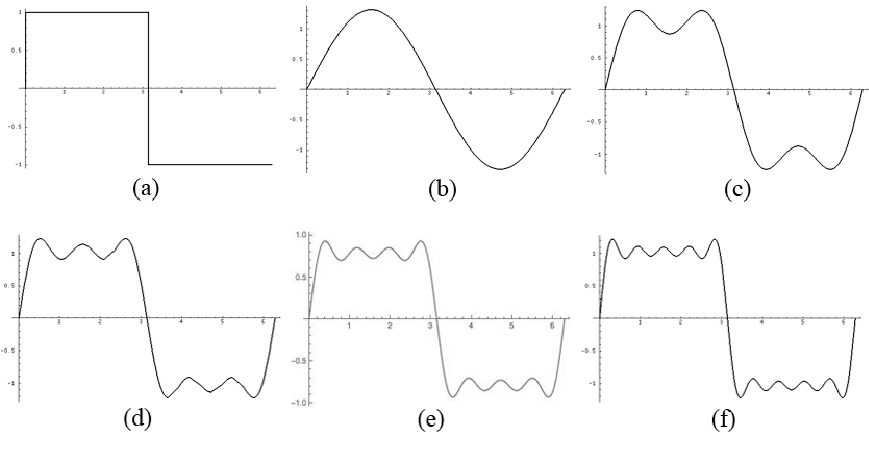
\includegraphics{images/fig-8}
\caption{\label{harmonics}Original square wave shown as (a). Successive FFT harmonic combinations used to reconstruct it: one, three, five, seven, and nine, shown as (b) to (f)}
\end{figure}

For complete fidelity, one would require an infinite number of odd harmonics (at frequencies $\omega, 3\omega, 5\omega�, 7\omega$, \textellipsis{} (2n+1)$\omega$ \textellipsis$\infty$). In real systems this is not practical. Figure \ref{harmonics}b through \ref{harmonics}f show the increasingly accurate representation of the square wave as additional harmonics are added to the representation. The residual ripple is the manifestation of the Gibbs phenomenon.

In DFT analysis, the bandwidth of an original analogue signal that has been sampled to provide the digital input must be limited by filtering before sampling and processing because frequency components higher than twice the sampling rate cannot be represented and will show up as aliasing---spurious frequency components arising from the inadequacy of the sampling rate. To approach fidelity, the sampling frequency must be \emph{at least} twice the highest frequency present in the input signal to avoid this aliasing---a minimum frequency known as the ``Nyquist'' frequency. Related topics belong within the field of communication theory, which was originally developed by Claude Shannon at the Bell Laboratories (Shannon 1951). It is still an ongoing and important area of research.

The TRM produces discrete samples at a rate that exceeds the Nyquist rate for the output signal representation but, since the DFT operates on a finite number of samples, spectral artefacts are still introduced. Windowing, is a sample weighting technique and as noted, provides a basis for mitigating the problem. A rectangular window is the worst since the waveform is arbitrarily truncated at the start and finish. Most of the other windows bring the weighting to zero at the start and end of the sample window. The Kaiser-Bessel and Hamming approaches include adjustable window parameters. There is some provision for adjusting the relevant parameters in the ``Analysis'' subsystem, as further detailed below.

\begin{figure}[htb]
\centering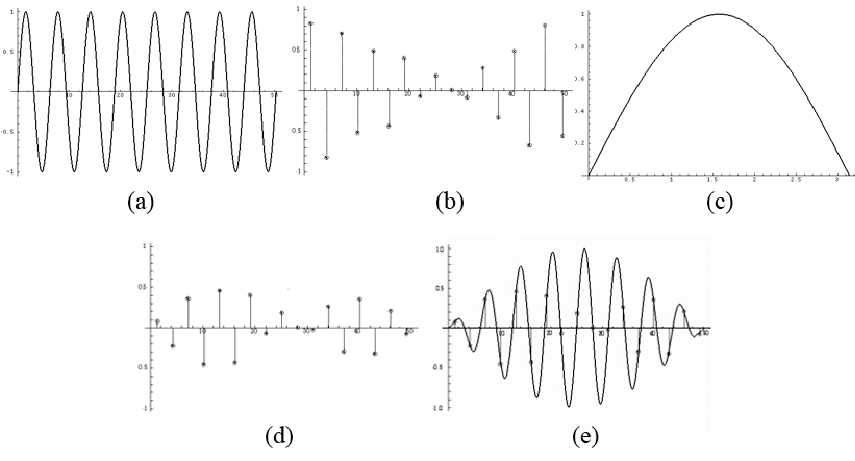
\includegraphics{images/fig-9}
\caption{\label{sampling}Sampling and reconstructing a sin wave, one window's worth}
\end{figure}

Figure \ref{sampling} shows a half-sin-wave-weighted set of samples of a steady sine wave of peak-to-peak amplitude -1 to +1. Figure 9(a) shows an analogue form of a continuous sin wave. Figure \ref{sampling}b shows the 17 Pulse Code Modulation (PCM) samples from the wave obtained by sampling at slightly over the Nyquist rate. The ``Bin size'' (number of samples in the window) is 17. ``Bin sizes'' are almost always powers of two or powers of two, plus one. However, note that the interaction between sampling frequency and the weighted waveform produces a non-intuitive representation with a largest sample value of only half the peak positive or negative values in the original waveform and seems to be the ``wrong shape''. This is simply how the samples fall relative to the waveform's changing amplitude. Figure \ref{sampling}c shows the weighting window. Finally Figure \ref{sampling}d shows the window-weighted set of PCM samples, and \ref{sampling}e shows the analog waveform reconstructed from those to give a window-weighted version of the original.

Different windows have an effect on any waveform that is reconstituted from the spectral description (by means of an Inverse Fourier Transform---possibly after some manipulation of the spectrum to simplify it or remove unwanted components). The interested reader should check the reference given above, or other web-based and text-book resources, because a full discussion is outside the scope of this manual. Like probability theory, the problems and solutions are not intuitively obvious. What has been presented should provide a reasonable basis for understanding and using the Tube Resonance Model by means of TRAcT---particularly the important matter of manipulating and understanding the Analysis sub-system output, which is the link between TRM configurations and its behaviour, though the user's ears are also important tools in evaluation.

\section{The TRAcT subsystems and their use}

\subsection{Starting}

Figure \ref{topo} shows the underlying topology of the TRM that is represented by the Resonant System window of Figure \ref{res-win}. The ``Tools'' drop-down menu from the menu bar of the OS X screen, when running TRAcT gives access to further subsystems: ``Control''; ``Open Monet Posture'' ; ``Glottal Source''; ``Noise Source''; ``Throat Transmission'' ; and ``Analysis''.

\begin{figure}[htb]
\centering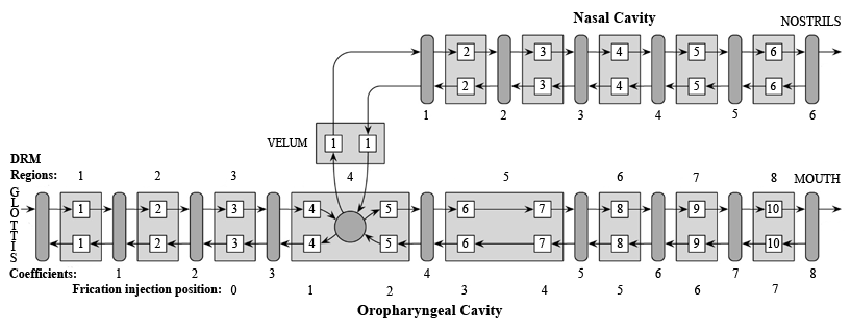
\includegraphics{images/fig-10-trm-topology}
\caption{\label{topo}The underlying Tube Resonance Model (TRM)}
\end{figure}

\begin{figure}[htb]
\centering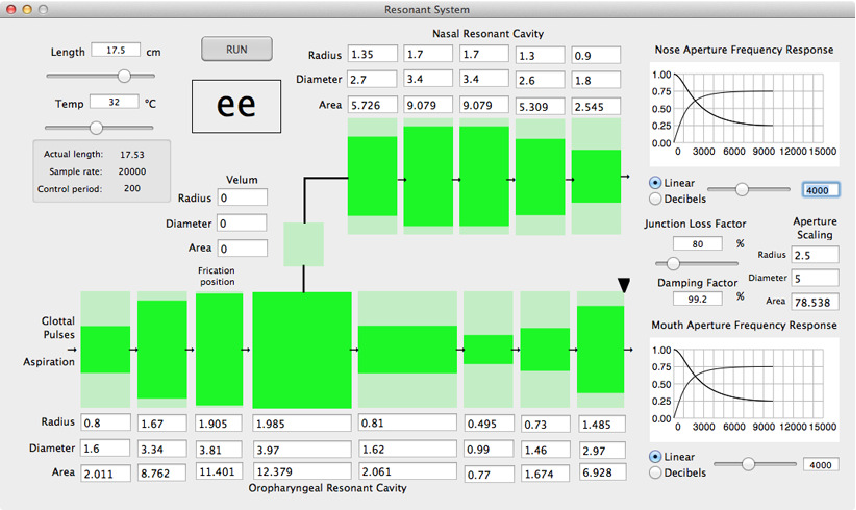
\includegraphics{images/fig-11-resonant-system}
\caption{\label{res-win}The resonance window}
\end{figure}

The Analysis sub-system has already been discussed in some detail. The remaining control panels are discussed in the following sections.

\subsection{The Resonant System}

The Resonant System panel appears with default values when first opened, as shown in Figure \ref{res-win}. The central feature is a representation of the eight DRM regions (tube sections), the velar opening, and the sections representing the nasal passages. Each has direct manipulation control for the radius of the appropriate section or passage, by dragging the edge, along with a display of the radius, diameter, and cross-sectional area.

The cross-sectional areas for the oro-pharyngeal (DRM) regions can be varied from roughly 0 to 12cm\textsuperscript{2}. The defaults for the nasal tube are set to reasonable values, whilst those for the oral tube represent an ``ee''-like sound (/i:/), and the velum is closed. The radii, diameters, and areas of any tube section, or the velar connection, may be changed, whether the TRM is producing sound or not, by either direct manipulation using the mouse to drag the edge of the section (or velar connection), or by entering one of the associated fields. It is usual to leave R1, the first---pharyngeal---section, alone, for technical reasons. It should perhaps, count as an control rate parameter, related to the ``speaker'' characteristics rather than than speech production rate---utterance rate---control. It is really fixed for an individual, and basically sets the scale for the rest of the tube sections. Note that if the Resonant System window is closed whilst  sound is being generated, TRAcT is liable to crash, due to its multithreaded operation.

When the TRM posture is determined by loading a Monet posture, the identity of the posture is shown as a label in the box below the ``Run/Stop'' button. Any change to an utterance-rate parameter deletes the label, with the exception of pitch. Also, changing the nose shape also deletes the label even though this is defined by control-rate parameters.

An unrestricted uniform tube, approximately 17 cm long and filled with air at normal temperature and pressure, produces resonant peaks (formants) at 500 Hz, 1500 Hz, 2500 Hz, 3500 Hz and so on (Flanagan 1972, pp 58-61). The frequencies are affected by temperature, pressure and the density of the gas in the tract. An extreme example of the effect of reduced density is so-called ``helium speech'' which occurs both as a dangerous party trick (by breathing helium a few times before speaking) and for divers breathing a helium/oxygen mixture to avoid problems with nitrogen bubbles in the blood (the ``bends''). With helium speech the resonances are much higher in frequency due to the lower density. The speaker sounds like a cartoon chipmunk and is quite hard to understand.

The TRM assumes normal air pressure and air density, but makes allowance for variation in temperature and length. These can be set using the fields and sliders at the top left of the Resonant System panel. The values actually used for computation may be slightly different so they are displayed below the fields/sliders. The air in the oral and nasal tubes is normally at a higher temperature than the ambient  air temperature.

An important factor in the behaviour of a tube resonator, and on the sound emitted, is the ``radiation impedance''---the impedance/admittance at the open end of both the oral and nasal tubes. The impedance affects how much energy is reflected back into the tube, and how much escapes (see Figure \ref{scatter}). The reflected energy enables the resonant behaviour of the tube, as explained by Julius Smith (see Section \ref{smith}). The length and other factors already mentioned are obviously also important. Modelling the radiation impedance for the human vocal tract is somewhat problematic and has not yet been completely resolved by research. Various models are have been proposed and used, including a piston in a wall (Flanagan 1972, p62), an aperture in a sphere of selected radius, and an aperture in an infinite baffle. The details of the model used for the TRM are not too important to the average user, but it is necessary to realise that two graphs and associated controls are provided at the right of the Resonant System panel to allow some adjustment of the properties of the oral and nasal apertures, controlling the frequency characteristics of the energy passed through the aperture (admittance) and the energy reflected back (impedance), both of which are plotted. These are the sub-panels Nose Aperture Frequency Response and Mouth Aperture Frequency Response. A control for varying the nominal aperture size---``Aperture Scaling''---is also provided.

\begin{wrapfigure}{L}{0.6\textwidth}
\centering
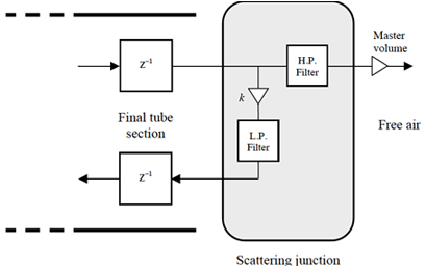
\includegraphics[width=0.55\textwidth]{images/fig-12}
\caption{\label{scatter}The scattering junction}
\end{wrapfigure}

The effect of increased radiation impedance on the formants of a uniform tube is to lower the frequency and increase the bandwidth of the formants (Flanagan 1972: 64). Losses at the glottis and through the (fleshy) cavity walls also affects the formants as do heat conduction and viscous losses. Some of these losses are lumped together as a ``Junction Loss Factor'' (affecting the transmission of energy between the tube segments, and controlled by the field and slider with that name); in addition Throat Transmission loss has its own panel (See section 3.4). The losses are frequency-dependent. Manzara (2005) summarises what happens at the open end of a resonating tube:

\begin{quote}
\footnotesize
``The frequency response of the reflected and radiated sound at the tube termination must also be modeled. This is done by using a fixed one-pole low-pass filter for the reflected pressure waves, and a fixed one-pole one-zero high-pass filter for the radiated sound [as shown in Figure 12]. Since the junction between the last tube section and free air is lossless, the frequency response of the radiation filter should be the exact inverse of the frequency response of the reflection filter. That is to say, any energy at a particular frequency that is not radiated should be reflected.''
\normalsize
\end{quote}

In the graphs provided, the top plot represents the reflected energy and the bottom plot the radiated energy, as approximated by the simple filters that are implemented.


\begin{wrapfigure}{R}{0.4\textwidth}
\centering
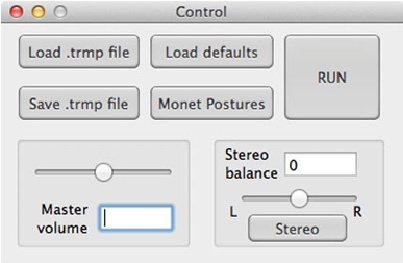
\includegraphics[width=0.35\textwidth]{images/fig-13}
\caption{\label{cont-pan}The Control panel}
\end{wrapfigure}


\subsection{The Control Panel}

The main ``Control'' panel---Figure \ref{cont-pan}---is self-explanatory. Two buttons on the left allow .trmp \footnote{The .trmp extension stands for ``tube resonance model parameters'', see Section \ref{trmp} }files representing the current TRM configuration to be saved and restored-both ``control rate'' and ``utterance rate'' parameters. The latter vary at a rate associated with Monet articulation (shape, pitch, noises \textellipsis) whilst the former represent characteristics of the speaker (tube length, tube losses, nose shape, \textellipsis). ``Load Defaults'' restores the TRM to its default configuration, whilst ``Monet Postures'' provides an alternate method of bringing up the ``Select Monet Posture'' window. The ``Run'' button on the right toggles between ``Run'' and ``Stop'' depending on the current run state of the TRM.

Below that are the ``Master Volume'' and ``Stereo balance'' controls, which perform the obvious functions, with control by slider or by entering new values in the display fields. Either ``Stereo'' or ``Mono'' may be chosen at the bottom left by a pull-down menu. These two controls are currently inactive.

\subsection{The Throat Transmission and Noise Source panels}

\begin{wrapfigure}{L}{0.4\textwidth}
\centering
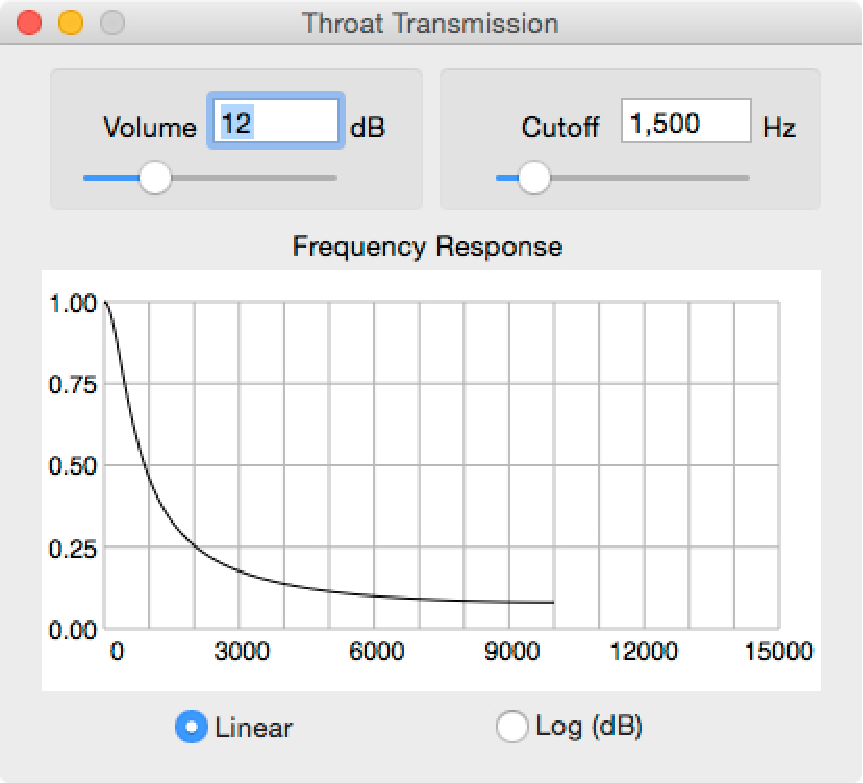
\includegraphics[width=0.35\textwidth]{images/fig-14-throat-transmission}
\caption{\label{throat}Throat transmission control}
\end{wrapfigure}

Figure \ref{throat} shows the Throat Transmission panel, with a graph of the loss frequency characteristic through the non-rigid walls of the throat. Since some energy passes through the soft tissues, this energy is radiated and becomes part of the output sound so a volume control for the amount radiated is provided. The transmission represents the portion of throat losses from the energy in the tube, and affects the resonances. The cutoff frequency can be varied and the graph plotted as either linear or log (dB). The latter option is currently inactive.

The ``Noise Source'' subsystem, Figure \ref{noise}, provides both aspiration noise and fricative noise, together with means of controlling them appropriately. Aspiration is random energy generated relatively low in the oro-pharyngeal tract mostly at the open, non-vibrating glottal folds, but also due to turbulent flow in the lower pharynx. The spectrum of aspiration is shaped by the resonant properties of the whole oro-pharyngeal tract and the source does not vary significantly in position or quality so that only a volume control is needed. The generation of ``breathy voice'' is covered in Section \ref{breathy}.

\begin{wrapfigure}{R}{0.6\textwidth}
\centering
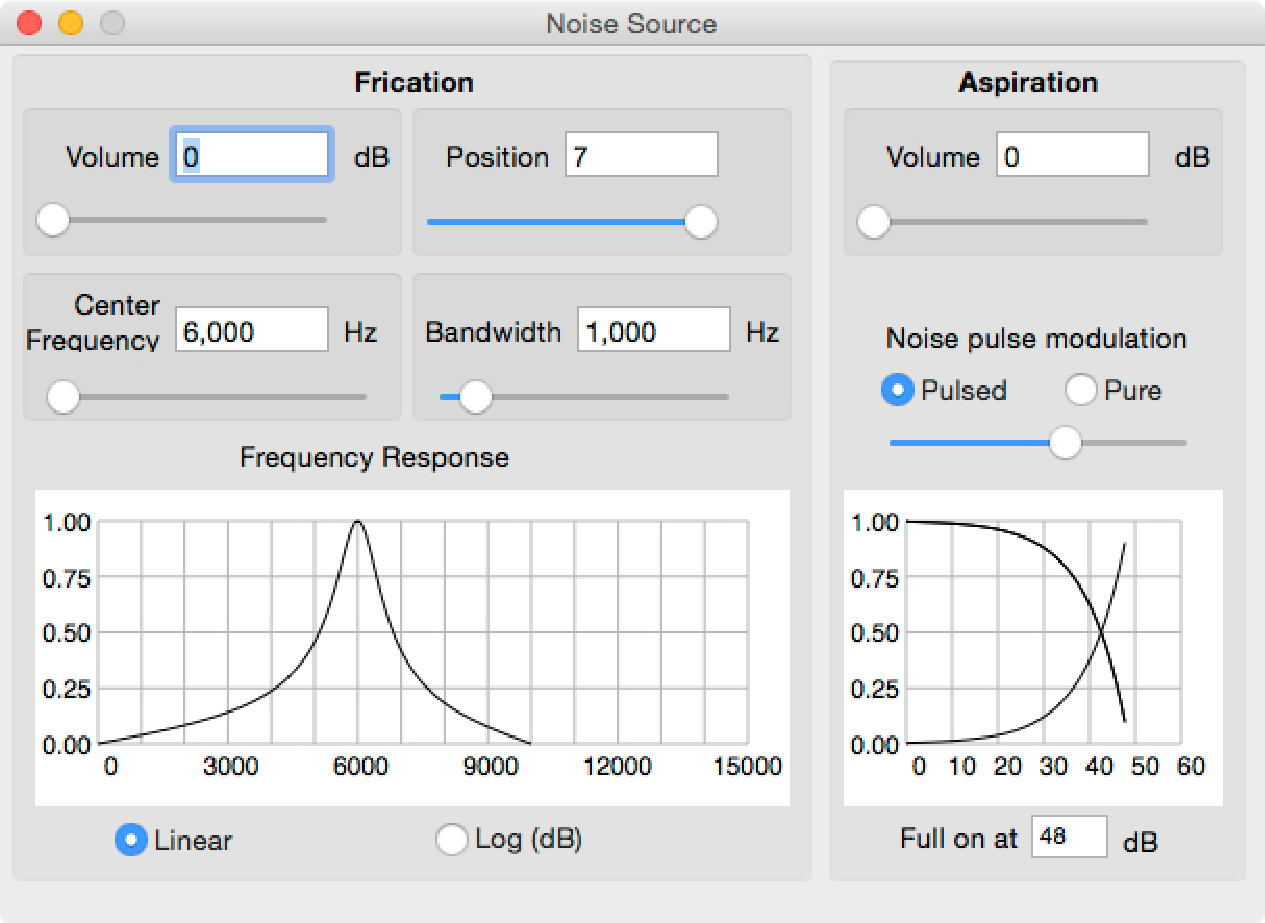
\includegraphics[width=0.55\textwidth]{images/fig-15-noise-source}
\caption[Noise source]{\label{noise}Noise source: fricative CF \& BW, aspiration \& breathy voice}
\end{wrapfigure}

Fricative noise arises at varying positions in the oro-pharyngeal tract, depending where the significant constriction producing the noise occurs (the place of articulation). The consequent turbulent airflow at the constriction gives different fricatives distinctive frequency characteristics, due in part to the filtering effect of the vocal tract. Sliders and fields are provided to set both frequency and bandwidth of the noise injected, and a display window shows the spectrum of the resulting noise with radio buttons to set either a linear or a logarithmic (dB) amplitude scale (currently only a linear display is active). In addition, a pulse modulation control is provided that allows the fricative noise to be modulated in amplitude at the pitch frequency. This allows better simulation of sounds like /z/ (the voiced alveolar fricative) in the middle of the word ``razor''. The level at which the noise is pulsed may be set by entering the appropriate dB value in the field or by the slider provided. The two plots for pure and pulsed noise change appropriately.

Finally, a slider and field are provided to set the ``Volume'' and ``Position'' for the fricative noise. ``Position'' determines where, along the oro-pharyngeal tract the noise is injected, which depends on which place of articulation is required. An arrow above the sectional representation of the DRM regions in the ``Resonant System'' display also moves to show the physical position that corresponds to the setting entered. Positions vary from DRM region R3 (0.0) (pharyngeal fricative)through to lips (DRM region R8-a bilabial fricative) (7.0). The place of injection is continuously variable because at places intermediate between the ends of a given section, the injected noise is split into two components, proportional to the division of the section, and injected appropriately at both ends of the section.

The parameters for fricative control are fairly minimal. Strevens (1960) studied the spectra of nine British English fricatives and found significant multi-peaked variation in spectra. The TRM approximates this variation by manipulating only the volume, centre frequency and bandwidth of a single FIR filter. In fact, when the noise is injected further back down the tract than the lips, the noise spectrum is shaped by the resonant properties of the portion of the tract involved, which is almost certainly responsible for at least some of the fricative spectra frequency peaks observed by Strevens (and others). Another advantage of the acoustic tube emulation is that natural transitions of the natural formant resonances cause appropriate movements of the fricative spectral peaks. Experience shows that these formant transitions associated with the dynamics of articulation are sufficiently powerful cues to fricatives that the detailed spectra are not all that important. In fact, telephone speech over band-limited telephones would not be possible if this was not true because most of the spectral quality is cut off completely (though ``f'' and ``s'' are frequently confused for exactly this reason, since the spectral cue is more important for this particular distinction). Fortunately the differences are reasonably simulated by the parameters we use. Ideally, given enough knowledge and computational power, the turbulent airflow at each partial closure associated with the different fricative articulations would be modelled accurately so that the base spectra would be appropriate. There is significant variation between the spectra of different individuals in real speech in any case.

\subsection{The Glottal Source}

The final subsystem to consider is the Glottal Source. The associated control panel is seen in Figures \ref{glot1} to \ref{glot4}. This panel controls the voicing energy (excitation) injected into the high-impedance end of the oro-pharyngeal tract, at the glottis, where the vocal folds (often loosely and incorrectly called ``vocal cords'') are located.

The volume flow through the glottis is roughly a triangular wave with a single discontinuity at closure which generally produces all harmonics of the fundamental glottal rate, falling off at roughly 12dB per octave with increasing harmonic frequency (remember, the dB scale is power-based with zero being an arbitrary reference power). This is what is displayed in the ``Harmonics'' sub-panel.

\subsubsection{Glottal Pulse Parameters}

\begin{figure}
\begin{minipage}{.55\textwidth}
\centering
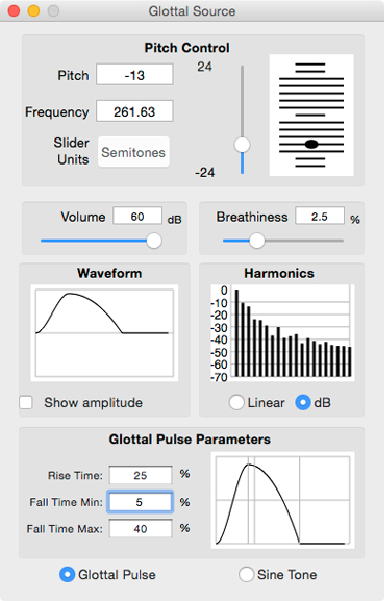
\includegraphics[width=0.55\textwidth]{images/fig-16-glottal-source-1}
\captionof{figure}{\label{glot1}The Glottal source panel:\\default set-up}
\end{minipage}%
\begin{minipage}{.55\textwidth}
%\hspace{-4cm}
\centering
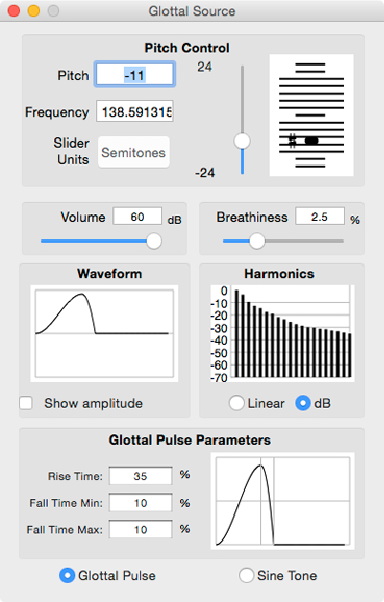
\includegraphics[width=0.55\textwidth]{images/fig-17-glottal-source-2}
%\hspace{-2cm}
\captionof{figure}{Rise/fall time \& \\ pitch change}
\label{glot2}
\end{minipage}
\end{figure}

The question of which artificial glottal pulse shape gives the most natural sounding voice has been a subject of research for decades. Our choice was the ``Rosenberg B'' waveform (which is almost identical in shape to ``Rosenberg C'') as seen in the ``Waveform'' sub-panel. As an aid to visualisation, the Rosenberg C waveform comprises of a raised half sine wave joined smoothly to a quarter sine wave at twice the amplitude. The ``Rosenberg B'' is made of polynomial functions and, as noted, is almost indistinguishable. Both ``B'' and ``C'' provide a smooth onset with a sharp termination (a single discontinuity in both first and second order derivatives). The ``B'' version was experimentally judged by listeners to produce the most natural voice quality when substituted for the original glottal pulse in speech recomposed from a decomposition of natural speech (Rosenberg 1971) and has a slightly sharper offset so a little more high frequency content than the ``C'' version (which was a close second). A total of six artificial glottal pulse shapes were tested. A second experiment looked at the rise and fall times of the ``C'' waveform. The defaults chosen for TRAcT are in the rise/fall region judged most natural in that experiment. The broader topic is usefully discussed in Witten (1982 pp 95-101) in connection with the excitation of formant synthesisers (which excite variable formant filters rather than a tube analogue). The fact remains that natural glottal excitation sounds better than even the best artificial glottal excitation, and also carries some speaker identification information.

\begin{figure}[htb]
\begin{minipage}{.55\textwidth}
\centering
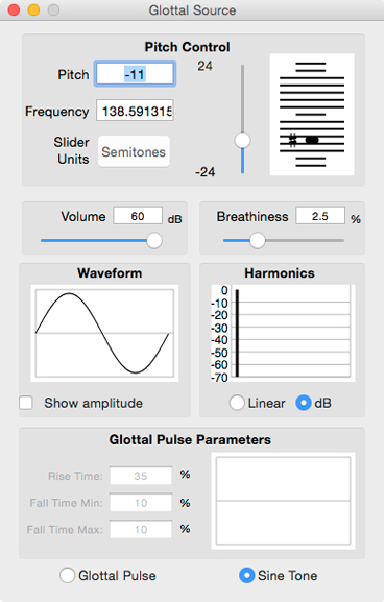
\includegraphics[width=0.55\textwidth]{images/fig-18-glottal-source-3}
\captionof{figure}{\label{glot3}Substituting \\a sine wave}
\end{minipage}%
\begin{minipage}{.55\textwidth}
%\hspace{-4cm}
\centering
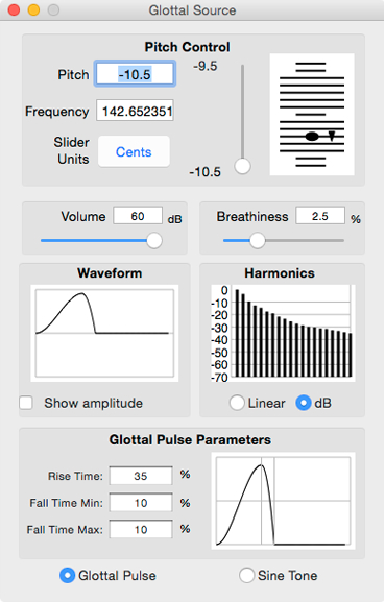
\includegraphics[width=0.55\textwidth]{images/fig-19-glottal-source-4}
%\hspace{-2cm}
\captionof{figure}{Changing \\pitch in cents}
\label{glot4}
\end{minipage}
\end{figure}


Ideally, given enough knowledge and computational power, a proper aerodynamic model of the vibrating vocal folds would be used to excite the TRM. We would expect this to improve the naturalness of the voice quality significantly. Vocal fold/glottis modelling is an active area of research. There was a conference on the topic in Marseille, France in August 2004 (Int. Conf. on Voice Physiology and Biomechanics August 18-20). Google ``vocal fold modeling'' to gain access to a wide variety of research.

The parameters of the glottal pulse-the rise and fall times-can be varied as a percentage of the total glottal period using fields within the ``Glottal Pulse Parameters'' sub-panel at the bottom. The maximum duration of the fall time can also be set---a value that is used during the wavetable calculations that create the amplitude-varying glottal pulse, effectively extending the fall period as the amplitude decreases, but limited by the maximum fall time set. The total range for all three time parameters is limited from 5\% to 50\% of the total period. The parameters also control a nominal pulse shape display to the right of the same sub-panel with a greyed line for the maximum and minimum fall times. Figure \ref{glot2} shows a situation in which the parameters have been changed from their default values. Note that the pitch pulse does not extend over the whole pitch period, the zero line represents the glottis in closure.

Immediately above the Glottal Parameters sub-panel lie the ``Waveform'' and ``Harmonics'' sub-panels which show the glottal pulse shape and the corresponding harmonic spectrum respectively. These respond to the glottal pulse parameter settings. If the radio buttons at the bottom of the main panel below the Glottal Pulse Parameters sub-panel are set to ``Sine Tone'' instead of ``Glottal Pulse'' the Waveform display changes to show a full cycle sine wave and the ``Harmonics'' display shows a single harmonic corresponding to the sine wave as shown in Figure \ref{glot3}. The sine wave input can be used for test purposes, sweeping a single frequency through a range to examine the tube response to a pure tone.

Provided the ``Show amplitude'' check box just below the Waveform display is checked, the changes in shape and variation in fall time can be seen by changing the ``Rise Time'', ``Fall Time Min.'' and ``Fall Time Max.'' settings and varying the ``Volume'' control just above the Waveform display. The ``Volume'' control changes the amplitude of the pulse. The change in duration of the fall as the amplitude changes can be seen more easily by not checking the box, because then the displayed amplitude does not change according to the actual pulse amplitude. The ``Show amplitude'' facility is currently inactive.

\subsubsection{Adjusting the pitch value}

The frequency of the glottal pulse, or sine wave, is set at the top of the main ``Glottal Source'' window using several controls, plus a display of the musical note equivalent of the pitch. ``Pitch'' field shows the TRM parameter value-which nominally varies between +24 and -24-directly, although this range does get slightly extended when necessary to allow adjustment in the ``Cents'' mode. ``Frequency'' shows the physical frequency corresponding to the pitch. Both ``Pitch'' and ``Frequency'' fields may be entered directly, or the vertical slider may be used to vary the pitch. Figure 17 shows a pitch adjustment away from the default value based on semitone adjustment. A sharp sign is added to the musical stave note as necessary. The full range occupies two octaves represented by the two staves. When in ``Cents'' mode (see the next paragraph). An up or down pointing arrow (Figure \ref{glot4}) shows when the pitch differs upwards or downwards from the nominal pitch represented by the musical note position (two staves). Changing the pitch or slider field after returning to ``Semitones'' mode, produces the expected change, but offset by the deviation in cents last in force.

The ``Slider Units'' toggle button allows ``Semitones'' or ``Cents'' to be selected as the units of change. The cent is a logarithmic interpolation within a semi-tone and provides 100 logarithmic steps per semitone. Thus there are 1200 cents per octave since an octave is 12 semitones. If ``Cents'' are selected, then, as the pitch value is changed, the range of movement by slider is restricted to one semi-tone and an up arrow or down arrow appears beside the musical note display according to whether the current setting is somewhat above or somewhat below the musical note displayed to a maximum of + 0.5 of a semitone. The frequency and pitch fields can still be entered normally. The musical scale is calibrated to A = 440 Hz (``Concert pitch'') so that middle C comes out at 261.63 Hz rather than the old-fashioned 256 Hz. This is done to allow a synthesised singing voice to match modern musical instruments.

\subsubsection{``Breathy Voice''}
\label{breathy}

The remaining control is ``Breathiness''---a slider and percentage display just below the musical note display. When real vocal folds are vibrating, they may not completely close at nominal closure for a variety of reasons. The commonest case is for female voice, in which the vocal folds only close for part of their length, allowing air-flow through the small triangular portion that remains open. This introduces a breathy noise (similar to light aspiration) during voiced sounds. The effect is characteristic of female speech and is called ``breathy voice''. Readers, especially male readers, must be aware of the appeal of a ``husky voice'' which is an extreme version of this consistent sex marker. The main reason for including this control is accurate rendition of different voices, especially the basic male, female and child voices. Breathiness is an important parameter (along with tube length) for this exercise. The parameter can be varied from 0 to 10\% of the excitation energy.

\section{Using TRAcT: ``Monet'' and the creation of .trmp data files}

\subsection{Introduction: relationship between ``Monet'' and ``TRAcT''}

\begin{figure}[htb]
\centering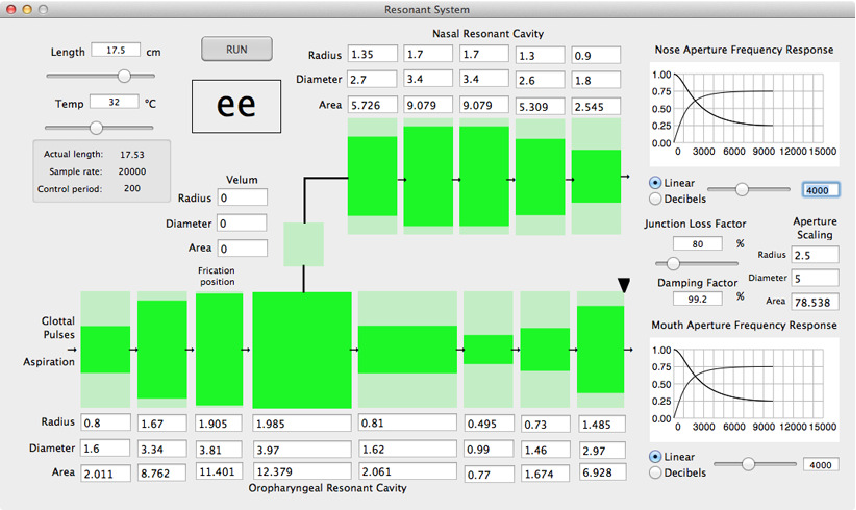
\includegraphics{images/fig-11-resonant-system}
\caption{\label{res-win2}The resonance window (again), set for an [i:] sound as in ``heed''}
\end{figure}

\begin{wrapfigure}{L}{0.5\textwidth}
\centering
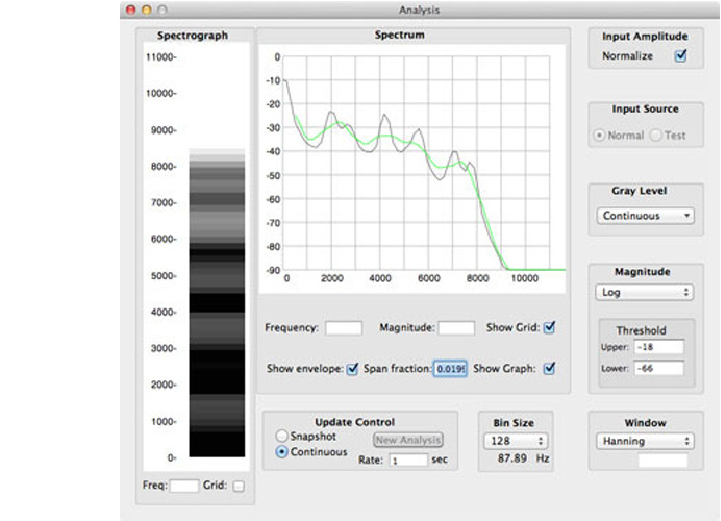
\includegraphics[width=0.45\textwidth]{images/analysis}
\caption{\label{anal2}A broad-band analysis of the [i:] sound by the TRAcT analysis system}
\end{wrapfigure}

As previously noted, TRAcT was an important tool, created to explore the vocal tract posture/sound space available from the TRM at the time when the posture databases needed for synthesising spoken English were being created, using the database creation and editing system ``Monet''. At the time, there were no comprehensive data on vocal tract configurations, or on the dynamics of combining successive articulatory postures together---``articulating'' the postures---to create intelligible speech. Even today, synthetic speech by computer is usually based on concatenating real speech segments (which requires large collections of recorded speech segments even for a single speaker), or using rules and data originally developed to drive formant synthesisers derived from the work in the 50s on formant values, fricative spectra and transitions, using direct measurements on spectrograms (DECTalk). Unlike formant synthesisers, the articulatory approach developed using Monet and TRAcT provides natural modelling of nasal effects and automatically produces the dynamics of higher formants rather than the lumped fixed approximations used in formant synthesisers. However, data in the form of vocal tract area cross sections is required. As noted, the ``Gnuspeech'' approach, employs an ``event based'' method of timing and placing parameter changes which allows great flexibility in placing where each individual parameter begins changing value, stops changing value, and what the values are, which is consistent with what happens in the articulation of natural speech. The required vocal tract area data was not generally available, and what was available was not related to the DRM regions at the start of the work.

Monet \footnote{Monet was the database creation component of the original software development. It is still incorporated as a major component of the Gnuspeech system but has changed its overll purpose somewhat to also provide convenient speech synthesis possibilities, including experiments with varied intonation contours. Several other applets that allow files to be spoken (BigMouth), speech parameters to be set in the operating system defaults database, and User and Application dictionaries to be created (PrEditor) have yet to be ported. See the Gnuspeech package that is part of this release.} allowed us to formalise, record and edit the underlying set of TRM postures representing the phonemes of English; and to discover the dynamic rules for compounding sequences of postures in a realistic approximation to the dynamics of articulation occurring naturally in human speech. Monet, as currently ported (thanks to Steve Nygard and Dalmazio Brisinda), provides means for speaking short utterances from text, preferably properly punctuated, and shows the annotated posture string-postures and formatting characters-derived from the input text. The composition includes models for rhythm and intonation according to rules based on research at the University of Calgary, based in turn on the work of David Abercrombie, Michael Halliday and Wiktor Jassem. The timing and values of the parameter tracks that are created to drive the TRM in producing speech can be displayed, together with the separately assigned pitch variation. Used all together in Gnuspeech, this creates the sounds, rhythm, and intonation of utterances.

This is all that will be discussed concerning the ``Monet'' system and its windows at this point, as a full discussion is beyond the scope of this manual, but it gives an outline as a basis for further discussion of TRAcT. Monet is fully documented in the manual that is part of this initial 0.9 release of Gnuspeech (GnuSpeech).

\subsection{Using the TRM to create ``postures''}

To set up the TRM configuration for a sound only requires that you have some knowledge of articulatory phonetics and can interpret this knowledge as tube radii and the expected spectral output. Appendix A provides a set of data for the entire nominal postural structure of spoken English (additional detail such as co-articulation and some acoustic events are taken care of by the composition rules also included in the Monet/GnuSpeech parameter generation system). As shown in Figure \ref{drm-map} the regions, starting at R1, correspond to: 1 to 3---the pharynx; 4---the region either side of the velum; 5---the back part of the oral cavity; 6---the front part of the oral cavity; 7---the region from the alveolar ridge to the teeth; and 8---the region from the teeth to the outside of the lips. Note that regions 4 and 5 are twice the length of the others, which are nominally 1.7 cm long for a 17 cm vocal tract.

Lip opening affects R8, as does lip protrusion (lip protrusion is not yet emulated in the model). Jaw rotation or tongue height (low to high) and position (back to front) affect R4 through R7 in constrained ways---a high back vowel, for example, leads to narrowing of R2 through R4, and opening of R6/7, whilst jaw rotation will affect R7 and R8 as well, with lip changes possibly reducing R8. A reasonable shape can be tried, preferably using articulatory data from the literature as a guide, and the effect can be checked by carrying out an analysis to determine the spectrum of the resulting sound. There is no precise data for the DRM control system, and the TRM control regions are not exactly aligned with these regions anyway. However, the match is close enough to get excellent results for synthetic speech with a low data rate, and a solid theoretical backing, compared to trying to control a 40-section tube model. Real vocal tracts vary, causing the matching of articulators with the ideal sections to be approximate anyway. We used a Kay ``Sonagraf'' for accurate determination of the spectra, but these days there are excellent spectrographic software tools {\footnote{For example, the Praat'' software already mentioned (Boersma 2001; van Lieshout 2003)} that are more detailed than the small-scale picture presented by the TRAcT ``Analysis'' system---which is really only a guide. An expandable frequency scale should be added to the ``Spectrum'' to provide more visible detail, and a better ``Continuous'' gray scale should be provided for the ``Spectrograph''.

Figure \ref{drm-const} shows the effect a constriction in any one of the eight DRM regions has on the frequency of each of the three lowest speech formants. It can be used as a guide when modifying the tube configurations to get a better spectral match to a given real sound. Vowel sounds are fairly straightforward. The data in Wells (1963) is a useful starting point for British English. The data published by Peterson and Barney (1952) is more appropriate to General American. Dealing with consonants, especially stop sounds, is more problematical since they may have no steady-state spectrum, or the spectrum may be masked by nasalisation, etc. However, knowing the apparent origins of the formant transitions---the ``locii'', and the place of articulation, provide an excellent guide, as can listening to the resulting postures in continuous speech synthesis. Green's paper (1959) and Liberman's paper (1955) are helpful in this respect while Strevens (1960) gives some feel for the fricative characteristics. There is a wealth of literature, most of it from earlier times. The papers cited give an entry into the literature that is likely to be helpful; but the task is likely to prove more difficult for any language for which the linguistic/phonetic knowledge is less comprehensive.

Figure \ref{res-win2} shows the resonant system configured to produce a sound similar to ``ee'' in English. Figure \ref{anal2} shows the broad band analysis of the resulting output. Note the low first formant, and relatively high formants 2 and 3, characteristic of this sound. If a slightly different ``ee-like'' sound were required, the constrictions could be modified, knowing their effect in different DRM regions illustrated above. Changes in pitch and breathiness and tube length could be tried for particular purposes such as mimicking female speech or child speech, and other parameters varied to listen to the effects of different conditions and see the spectral effects of changes that changed the spectrum. Then the .trmp file\footnote{Actually a .trm file at the time} could be saved (see Section\ref{trmp}), and later transferred into the ``Monet'' system, where the sound could be tried as part of continuous speech in the language under consideration, listening to the result and performing a spectrographic analysis to understand the effect ``in context''. This also highlights the fact that, for successful database creation, TRAcT and Monet interact and must be used iteratively and in concert, with spectrographic hardware or software for accurate analysis.

Note that only the parameters affecting the individual sound---all but one of the ``utterance rate" parameters---would be saved and transferred. Although pitch is also an utterance rate parameter, it is necessarily managed separately from the TRM postures within the Monet system (except for micro-intonation special events). A number of parameters---the so-called ``control rate'' parameters mentioned above-do not vary from posture to posture (for example, tube length, temperature, basic pulse shape, mouth and nose aperture frequency responses, noise cross-mix, throat transmission, and junction loss factor).

Even the durations of the speech postures are outside the scope of TRAcT. Posture durations control rhythm, which is modelled as part of the Monet system along with the pitch variations that control intonation. Rhythm and intonation interact to create ``prosody''-the so-called ``suprasegmental'' aspects of speech. Prosody, as previously noted, directly and significantly affects meaning. A full discussion of the issues is outside the scope of this manual, but some insight into the approach taken for the gnuspeech text-to-speech system may be gained from reports related to research at the U of Calgary, and other places, that underpins the system prosody (e.g.~Halliday 1970; Hill 1978; Jassem, et al. 1984; and Taube-Schock 1993), and from the Monet manual that is part of this release.

\begin{wrapfigure}[18]{R}{0.35\textwidth}
\centering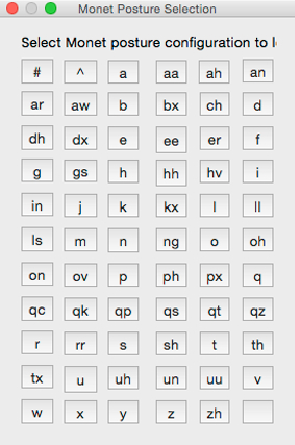
\includegraphics[width=0.3\textwidth]{images/monet-postures}
\caption{\label{mon-pos}The Monet Postures panel}
\end{wrapfigure}


The various static controls, such as ``Glottal Source'' waveform, ``Throat Transmission'', and ``Mouth/Nose Aperture Frequency Responses'' are generally best left at their default values, unless you have a particular objective in mind. The effects can be tried, of course, for interest. The one exception is the ``Pitch'' frequency. It is sometimes easier to hear the quality of the sound, for listening tests, with a value that is different from the default value. The author prefers a lower value.

The Noise Crossmix is of use in sounds such as /z/, where the combination of vibrating vocal folds and vocal tract constriction produce both voicing, and a modulation of the fricative noise.

\subsection{.trmp data \& Monet postures}
\label{trmp}

\subsubsection{Saving and restoring .trmp data}

If the user has created a posture using TRAcT, and wishes to save the work, the ``Save .trmp file'' button on the ``Control'' window, Figure \ref{cont-pan}, brings up a ``Save'' panel and allows the user to save the current working .trmp file. The .trmp files may be transferred into the Monet system later, to allow saved postures to be reloaded. Future improvements will allow better handling of file names, extensions and transfers. At present, the file name always has to be entered, and the extension is not protected, so can be erased or altered.

\subsection{Setting up Monet Postures}
\label{mon-pos-txt}



A recent addition to the TRAcT facilities has been the ``Monet Posture Selection'' window, shown in Figure \ref{mon-pos}. The window provides a matrix of buttons, each one calling up the posture indicated, allowing any one of the current ``Monet'' postures to be easily loaded into TRAcT for comparison and modification, or to provide the staring point for a new posture. To preserve the integrity of the current Monet posture file, the resulting new or modified postures can only be saved as a .trmp file.

\section{Help facilities available}

This on-line manual provides the only help facilities currently available. It should be integrated as a component of the TRAcT system in the form of on-line help.

\section{Acknowledgements}

The author wishes to acknowledge the fundamental work performed by Leonard Manzara in designing and implementing both the Tube Resonance Model itself and the original ``Synthesizer'' Graphical User Interface whilst he was a member of the Trillium R\&D group, as well as my research group at the University of Calgary. Len was our knowledgeable liason with Julius Smith and Perry Cook at CCRMA. Equal thanks are due to Craig Schock, also a member of both groups, for his insightful ``Monet'' implementation, which is the creative embodiment of the event-based model of speech that has long formed the basis of my speech research. There are others who made crucial contributions. Steve Nygard was involved in the original research at the University of Calgary, and has spent many months since as a volunteer on the port of ``Monet'' to the Macintosh, under OS X, as well as supporting the author's work on the ``Synthesizer'' port to what has now become ``TRAcT''.  Dalmazio Brisinda, who also worked with me at the university also put in very significant volunteer effort on the port of ``Monet''. Only some of the database creation components remain to be completed, mostly those parts responsible for writing the various database components after they have been edited.

Others who made important contributions to the research base that led to the creation of gnuspeech include Wiktor Jassem, Ian Witten, Julius Smith, Perry Cook, Ren\'e Carr\'e, Vince Demarco, David Marwood, Eric Zoerner, Michael Forbes, the Savannah Hackers, and Marcelo Matuda (the latter got the system running under GnuStep on Linux, and also simplified CMake-based multi-platform-based versions). A more detailed account of the contributions of these individuals, and others, appears on the project home page at: \href{http://www.gnu.org/software/gnuspeech/}{http://www.gnu.org/software/gnuspeech/ under ``Thanks to those who have helped''.}

\section{References}

ATAL, BISHNU S \& SL HANAUER (1971) Speech analysis and synthesis by linear prediction of the speech wave, J Acoust Soc Amer, 50 (2), Aug, pp 637-633.

ALLEN, JONATHAN, M. SHARON HUNNICUTT \&  DENNIS KLATT (1987) From text to speech: the MITalk system. Cambridge University Press, ISBN 0-521-30641-8, 216 pp

BOERSMA, PAUL 2001. \href{http://www.fon.hum.uva.nl/praat/}{\emph{Praat, a system for doing phonetics by computer}}. \emph{Glot International} 5:9/10, 341-347, accessed 2014-01-24)

CARRE, REN\'E \& SAMIR CHENNOUKH (1993) Vowel-Consonant-Vowel modeling by superposition of consonant closure on Vowel-to-Vowel gestures 3rd Seminar on Speech Production: Models and Data, Saybrook Point Inn May 11-13 1993

CARRE, REN\'E, SAMIR CHENNOUKH \& MOHAMAD MRAYATI (1992) Vowel-consonant-vowel transitions: analysis, modeling and synthesis Proc ICSLP 92 (Int. Conf. of Spoken Language Processing, Banff, Alberta, pp 819-822

CARRE, R \& MRAYATI, M (1994) Vowel transitions, vowel systems, and the Distinctive Region Model. in Levels in Speech Communication: Relations and Interactions. Elsevier: New York

CARRE, REN\'E, BJORN LINDBLOM \& PETER MACNEILAGE (1994) Acoustic contrast and the original of the human vowel space Acoust Soc Amer meeting, Cambridge MA, paper 3pSP

COOK, PERRY R (1991) Identification of control parameters in an articulatory vocal tract model with applications to the synthesis of singing. PhD Thesis, Stanford University, Dept of Electrical Eng, September

DUNN, HK (1950) The calculation of vowel resonances, and an electrical vocal tract J Acoust Soc Amer. 22 pp 740-753

FANT, C GUNNAR M \& S PAULI (1974) Spatial characteristics of vocal tract resonance mod es. SCS 74 (Speech Communication Seminar, Stockholm, Aug 1-3 1974, pp 121-133

FANT, C GUNNAR M (1956) On the predictability of formant levels and spectrum envelopes from formant frequencies. In For Roman Jakobson. Mouton: The Hague, 109-120

FANT, C GUNNAR M (1960) Acoustic theory of speech production. Mouton: The Hague

FANT, C GUNNAR M \& PAULI, S (1974) Spatial characteristics of vocal tract resonance models. Proceedings of the Stockholm Speech Communication Seminar, KTH, Stockholm, Sweden

FLANAGAN, JAMES L (1972) Speech analysis, synthesis and perception. Springer-Verlag: New York, ISBN 0-387-05561-4, 444 pp (Second Edition)

GREEN, PETER S (1959) Consonant-vowel transitions: a spectrographic study. Travaux de l'Institut de Phon\'etique de Lund, (also in Studia Linguistica XII 1958 number 2) (available in the Essex University library, UK)

HALLIDAY, MICHAEL A K (1970) A course in spoken English: intonation. Oxford University Press 134pp

HECKER, MHL (1962) - Studies of nasal consonants with an articulatory speech synthesiser. J Acoust Soc Amer 34, (2), February

HILL, DAVID R (1978) Some results from a preliminary study of British English speech rhythm Research report 78/26/5, Dept of Comp Sci, U of Calgary, 24 pp

HILL, DAVID R, LEONARD MANZARA \& CRAIG-RICHARD TAUBE-SCHOCK (1995) Real-time articulatory speech-synthesis-by-rules. Proc. AVIOS '95 14th Annual International Voice Technologies Conf, San Jose, 12-14 September 1995, 27-44.

HILL, DAVID R (1991) \href{http://pages.cpsc.ucalgary.ca/~hill/papers/conc/index.htm}{\emph{A conceptionary for speech and hearing in the context of machines
and experimentation}}, \url{http://pages.cpsc.ucalgary.ca/~hill/papers/conc/index.htm}, accessed 2015-05-06, Dept. of Computer Science, U of Calgary, report, 2nd edition 2004.

JASSEM, WIKTOR, DAVID R HILL \& IAN H WITTEN (1984) Isochrony in English speech: its statistical validity and linguistic relevance in Intonation, Accent and Rhythm: studies in discourse phonology (D Gibbon \& H Richter, eds), de Gruyter: Berlin \& New York, ISBN 3-11-009832-6

LAWRENCE, WALTER (1953) The synthesis of speech from signals which have a low information rate. In Communication Theory, Butterworth: London, 460-469

LAWRENCE, WALTER (1954) The experimental synthesis of speech from parameters Signals Research and Development Establishment Report: Christchurch, UK

LIBERMAN, ALVIN M, PIERRE DELATTRE \& FRANKLIN S COOPER (1955) Acoustic locii and transitional cues for 34 consonants J Acoust Soc Amer 27 (4), July

LIBERMAN, ALVIN M, FRANCES INGEMANN, LEIGH LISKER, PIERRE DELATTRE, P \& FRANKLIN S COOPER (1959) Minimal rules for synthesising speech. J Acoust Soc Amer 31 (11), 1490-1499, Nov

van LIESHOUT, PASCAL (2003)  \href{http://web.stanford.edu/dept/linguistics/corpora/material/PRAAT_workshop_manual_v421.pdf}{PRAAT: short tutorial: a basic introduction. \linebreak{}\footnotesize{http://web.stanford.edu/dept/linguistics/corpora/material/PRAAT\_workshop\_manual\_v421.pdf}} University of Toronto, Graduate Department of Speech-Language Pathology, Faculty of Medicine, Oral Dynamics Lab(accessed 2015-07-11)

MANZARA, LEONARD (2005) The Tube Resonance Model Speech Synthesizer. Poster paper : 149th Meeting of the Acoustical Society of America, Vancouver Hyatt Regency Hotel, Vancouver, British Columbia, Canada, May 16--20, 2005

MARKEL, JOHN D \& AUGUSTINE H GRAY (1976) Linear Prediction of Speech Springer-Verlag: New York, ISBN 3-540-07563-1

\"OHMAN, SEG (1966) Coarticulation in VCV utterances: Spectrographic measurements. Journal of the Acoustical Society of America, 39, pages 151-168

PETERSON, GEORGE E \& HL BARNEY (1952) Control methods used in the study of vowels J. Acoust Soc Amer 24 (3), 175-184, March. (Also Bell Monograph 1982)

POTTER, RALPH K, GEORGE A KOPP \& HARRIET G KOPP (1966) Visible Speech Bell Telephone laboratories: Murray Hill, New Jersey (Dover edition, LCCCN 65-23130, originally published in 1947, before Harriet Green had married George Kopp, so the authors were Potter, Kopp and Green for the orignial edition)

ROSENBERG, AE (1971) Effect of glottal pulse shape on the quality of natural vowels J Acoust Soc Amer 49 583-590

TAUBE-SCHOCK, CRAIG-RICHARD (1993) Intonation for computer speech output MSc Thesis, Dept of Comp Sci, U of Calgary, September (available from University Microfilms) (note this is the same person as ``Craig Schock'')

SHANNON, CLAUD (1948) The mathematical theory of communication Bell System Technical Journal, July \& October

SMITH JULIUS O III (2004)  \href{https://ccrma.stanford.edu/~jos/pasp/}{Physical audio signal processing}\\ \url{https://ccrma.stanford.edu/~jos/pasp/} accessed 2015-08-25

STEVENS, KEN, S KASOWSKI \& C GUNNAR M FANT (1953) An electrical analog of the vocal tract J Acoust Soc Amer 25 pp 743-742

STREVENS, PETER (1960) Spectra of fricative noises in human speech Language \& Speech, 3 (1), Jan/Mar

TOLKIEN JOHN RR (1966) The Return of the King George Allen \& Unwin: London, UK (Unwin Paperbacks 1978 combined edition ISBN 0-04-823229-7, page 620: Pippin speaking to Gandalf as he is carried away from his encounter with the Palant\"i�r at Orthanc, read by David R. Hill; and analysed by Neal Reid under the NRC of Canada grant A5261)

WELLS, JOHN C (1963) A study of the formants of the pure vowels of British English Progress Report, University College, London, UK, July

WHITFIELD, IC \& EF EVANS (1965) Behaviour of Neurones in the unanaesthetised auditory cortex of the cat J. Neurophysiology 28, 655-672

WITTEN IAN H (1982) Principles of Computer Speech Academic Press: London, ISBN 0-12-760760-9, 286 pp

\appendix

\section{Parameter data for Monet postures as derived, in part, by using ``TRAcT''}
\subsection{Introduction}

The TRM parameter data for the 65 or so articulatory postures that follow were experimentally derived during the last three months of 1994, using the original ``Synthesizer'' tool by the author and Leonard Manzara working together. More detail concerning the derivation should appear in a paper in preparation, but, briefly, it involved: (1) analysis of real speech using a Kay Sonagraf and the Sonagram App on the NeXT computer; (2) use of real speech data from publications such as Wells' vowel data (Wells 1963); (3) the adjustment of the DRM regions and other parameters in the Tube Resonance Model using Synthesizer, starting from a knowledge of articulatory phonetics and the effect of constrictions in the eight DRM regions on formant frequencies; (4) the fact that the vocal tract has structural and dynamic constraints on the configurations that are possible; (5) the analysis of the TRM output using the Analysis sub-system of Synthesizer and a comparison of this with the analyses from real speech (As in (1) above); and (6) the use of the Monet system to test the effectiveness of the postures derived, in continuous synthetic speech, by listening to a good variety of phonetic contexts, both monosyllables and connected speech.

Development of the ``Monet'', context rules, rewrite rules and the pronouncing dictionary proceeded in parallel. Steps were iterated as necessary. Rewrite rules allow the of ``special'' postures-for example: when a final /i/ precedes an initial /i/ a glottal stop must be inserted (a word juncture effect).

It will be noted that the R1 DRM region is always set to a 0.8 cm radius. In fact it probably need not have been included as a varying parameter because it really only determines the relative scale. Similar results could be obtained for all postures with different values of R1 leading to different, but geometrically similar values of the other 7 regions for each posture. This is presently an untested hypothesis, but one in which we have considerable confidence.

Region R1 corresponds to the first DRM region above the glottis. Region R8 corresponds to the last region, the teeth to the front of the lips leading to the mouth orifice itself. In some postures, the fricative spectral parameters (fricVol, fricPos, fricCF and fricBW) are set, with the fricative volume (fricVol) at zero. This is because the particular posture is associated with a fricative noise burst in which the fricative volume is controlled by a special event parameter profile rather than the regular parameter control using the fricative volume value. The fricative volume parameter settings are generally rather low. The noise balances within the TRM implementation need some attention. It causes some problems in the parameter displays within the Monet system because the values are hardly visible at values which give acceptable output energy, which also makes adjusting fricatives-especially voiced fricatives-during database creation somewhat tricky, especially for the placement and volume of special events.

The velum ``closed'' value default is 0.1 -- very slightly open. The same is true of closure for /t,d,k,g/ at their points of articulation (R6), /k,g/ (R5), and lip closure for /b,p/. It is a stratagem to avoid spurious artifacts.

It is important to realise that perceiving TRM postures is both static and dynamic. Vowels, which can be represented as a stand-alone steady state sound without losing any of their identity, can be heard when the TRM posture (articulation) is appropriately set up, though the ear and brain soon become habituated to the noise which begins to lose its identity. Short bursts of the sound are more convincing, but still lack the dynamic variation of real speech. However, when you come to steady state consonant postures (articulations), many of the cues we use in perceiving them are simply absent because the cues are dynamic-changes in formant frequency, or fricative characteristics as the sound approaches and leaves the posture, plus characteristic noise bursts.

Some consonant postures preclude any sound because the oro-pharyngeal and nasal passages are completely closed, though some sound may escape for a short time through the throat tissues if the vocal folds are vibrating---as in continuous speech, and the elasticity of the tissues allows some air flow to do this---the so called ``voice bar'' in the ``Visible Speech'' terminology of Potter, Kopp \& Kopp (1966). If the closure is maintained, the flexible parts of the tract fill up and air can no longer flow, so the vocal folds stop vibrating. Consonant postures can really only be tested as part of continuous speech, which is what we had to do. The locus theory of consonant perception (Liberman 1955, for example) derives from this essential basic fact. To the extent that such locii (the frequencies from which or to which formant transitions appear to move in speech spectrograms) exist, they are related to the postures associated with the consonants. The phenomenon of co-articulation---the influence of context on the actual configuration in continuous speech---ensures that there are no fixed locii for consonants any more than there are fixed formant combinations for vowels. However, there is more than a grain of truth in the concept of consonant locii. The GnuSpeech system context rules are designed to allow such co-articulation effects to be included. Green (1959) provides a comprehensive spectrographic study of consonant-vowel transitions.

The pronunciations associated with the posture symbols below, which were designed to be mnemonic and easily typed, have also been rendered in terms of both the International Phonetic Association and Webster's phonetic symbols, together with other helpful information, in an on-line pronunciation guide. Note that only one version of each posture is provided. The nominal marked, unmarked and other (e.g. syllabic) versions have the same TRM parameter values. Only the durations differ. Durations are relevant at the Monet/GnuSpeech level of continuous speech, rather than at the TRM level. Also, as already noted, some acoustic characteristics (for example, bursts of aspiration or fricative noise, and co-articulation effects) of the sounds are managed by the rules and prototypes in the Monet/GnuSpeech system and are, as far as the TRM is concerned ``hidden''.

\subsection{Micro-intonation and tube section radii for the ``Monet'' postures}

\begin{footnotesize}
(Note: This is the complete raw posture data contained in the GnuSpeech database. The Monet Manual, Appendix D contains the equivalent formant and timing data. Since the timing data varies between marked and unmarked versions of a given posture, each posture has two entries in that table.)
\end{footnotesize}

\begin{scriptsize}
\noindent\begin{center}\begin{tabular}{|c|cccccccc|}
\hline
& & & & \textbf{Parameter}  &  &  &  &\\

\hline

\textbf{Phone} & \textbf{microInt} & \textbf{glotVol} & \textbf{aspVol} & \textbf{fricVol} & \textbf{fricPos} & \textbf{fricCF} & \textbf{fricBW} & \textbf{velum}\\
&\textbf{r1} & \textbf{r2} & \textbf{r3} & \textbf{r4} & \textbf{r5} & \textbf{r6}& \textbf{r7} & \textbf{r8}\\
\hline
\#& 0.0 & 0.0 & 0.0 & 0.0 & 5.5 & 2500.0 & 500.0 & 0.1\\
& 0.8 & 0.89 & 0.99 & 0.81 & 0.76 & 1.05 & 1.23 & 0.01\\
\hline
$\wedge$& 0.0 & 0.0 & 0.0 & 0.0 & 5.5 & 2500.0 & 500.0 & 0.1\\
& 0.8 & 0.89 & 0.99 & 0.81 & 0.76 & 1.05 & 1.23 & 0.01\\
\hline
a & 0.0 & 60.0 & 0.0 & 0.0 & 5.5 & 2500.0 & 500.0 & 0.1\\
& 0.8 & 0.65 & 0.65 & 0.65 & 1.31 & 1.23 & 1.31 & 1.67\\
\hline
aa & 0.0 & 60.0 & 0.0 & 0.0 & 5.5 & 2500.0 & 500.0 & 0.1\\
& 0.8 & 0.65 & 0.84 & 1.15 & 1.31 & 1.59 & 1.59 & 2.61\\
\hline
ah & 0.0 & 60.0 & 0.0 & 0.0 & 5.5 & 2500.0 & 500.0 & 0.1\\
& 0.8 & 0.65 & 0.45 & 0.94 & 1.1 & 1.52 & 1.46 & 2.45\\
\hline
an & 0.0 & 60.0 & 0.0 & 0.0 & 5.5 & 2500.0 & 500.0 & 1.5\\
& 0.8 & 0.52 & 0.45 & 0.79 & 1.49 & 1.67 & 1.02 & 1.59\\
\hline
ar & 0.0 & 60.0 & 0.0 & 0.0 & 5.5 & 2500.0 & 500.0 & 0.1\\
& 0.8 & 0.52 & 0.45 & 0.79 & 1.49 & 1.67 & 1.02 & 1.59\\
\hline
aw & 0.0 & 60.0 & 0.0 & 0.0 & 5.5 & 2500.0 & 500.0 & 0.1\\
& 0.8 & 1.1 & 0.94 & 0.42 & 1.49 & 1.67 & 1.78 & 1.05\\
\hline
b & -2.0 & 43.5 & 0.0 & 0.0 & 7.0 & 2000.0 & 700.0 & 0.1\\
& 0.8 & 0.89 & 0.76 & 1.28 & 1.8 & 0.99 & 0.84 & 0.1\\
\hline
ch & -2.0 & 0.0 & 0.0 & 0.0 & 5.6 & 2500.0 & 2600.0 & 0.1\\
& 0.8 & 1.36 & 1.74 & 1.87 & 0.94 & 0.0 & 0.79 & 0.79\\
\hline
d & -2.0 & 43.5 & 0.0 & 0.0 & 6.7 & 4500.0 & 2000.0 & 0.1\\
& 0.8 & 1.31 & 1.49 & 1.25 & 0.76 & 0.1 & 1.44 & 1.3\\
\hline
dh & -1.0 & 54.0 & 0.0 & 0.25 & 6.0 & 4400.0 & 4500.0 & 0.1\\
& 0.8 & 1.2 & 1.5 & 1.35 & 1.2 & 1.2 & 0.4 & 1.0\\
\hline
e & 0.0 & 60.0 & 0.0 & 0.0 & 5.5 & 2500.0 & 500.0 & 0.1\\
& 0.8 & 0.68 & 1.12 & 1.70 & 1.39 & 1.07 & 1.05 & 2.06\\
\hline
ee & 0.0 & 60.0 & 0.0 & 0.0 & 5.5 & 2500.0 & 500.0 & 0.1\\
& 0.8 & 1.67 & 1.91 & 1.99 & 0.81 & 0.495 & 0.73 & 1.49\\
\hline
er & 0.0 & 60.0 & 0.0 & 0.0 & 5.5 & 2500.0 & 500.0 & 0.1\\
& 0.8 & 0.89 & 0.99 & 0.81 & 0.76 & 1.04 & 1.23 & 1.12\\
\hline f & -1.0 & 0.0 & 0.0 & 0.5 & 7.0 & 3300.0 & 1000.0 & 0.1\\
& 0.8 & 0.89 & 0.9 & 0.81 & 0.76 & 0.89 & 0.84 & 0.5\\
\hline
\end{tabular}


\noindent\begin{tabular}{|c|cccccccc|}
\hline
& & & & \textbf{Parameter}  &  &  &  &\\

\hline

\textbf{Phone} & \textbf{microInt} & \textbf{glotVol} & \textbf{aspVol} & \textbf{fricVol} & \textbf{fricPos} & \textbf{fricCF} & \textbf{fricBW} & \textbf{velum}\\
&\textbf{r1} & \textbf{r2} & \textbf{r3} & \textbf{r4} & \textbf{r5} & \textbf{r6}& \textbf{r7} & \textbf{r8}\\
\hline



\hline g & -2.0 & 43.5 & 0.0 & 0.0 & 4.7 & 2000.0 & 2000.0 & 0.1\\
& 0.8 & 1.7 & 1.3 & 0.99 & 0.1 & 1.07 & 0.73 & 1.49\\
\hline gs & 0.0 & 0.0 & 0.0 & 0.0 & 5.5 & 2500.0 & 500.0 & 0.1\\
& 0.8 & 0.8 & 0.8 & 0.8 & 0.8 & 0.8 & 0.8 & 0.8\\
\hline h & 0.0 & 0.0 & 10.0 & 0.0 & 5.5 & 2500.0 & 500.0 & 0.1\\
& 0.8 & 0.8 & 0.8 & 0.8 & 0.8 & 0.8 & 0.8 & 0.8\\
\hline hh & 0.0 & 0.0 & 10.0 & 0.0 & 1.0 & 1000.0 & 1000.0 & 0.1\\
& 0.8 & 0.24 & 0.4 & 0.81 & 0.76 & 1.05 & 1.23 & 1.12\\
\hline hv & 0.0 & 42.0 & 10.0 & 0.0 & 5.5 & 2500.0 & 500.0 & 0.1\\
& 0.8 & 0.8 & 0.8 & 0.8 & 0.8 & 0.8 & 0.8 & 0.8\\
\hline i & 0.0 & 60.0 & 0.0 & 0.0 & 5.5 & 2500.0 & 500.0 & 0.1\\
& 0.8 & 1.05 & 1.57 & 1.75 & 0.94 & 0.68 & 0.79 & 1.12\\
\hline in & 0.0 & 60.0 & 0.0 & 0.0 & 5.5 & 2500.0 & 500.0 & 1.5\\
& 0.8 & 0.65 & 0.84 & 1.15 & 1.31 & 1.59 & 1.59 & 2.61\\
\hline j & -2.0 & 48.0 & 0.0 & 0.0 & 5.6 & 2500.0 & 2600.0 & 0.1\\
& 0.8 & 1.36 & 1.74 & 1.87 & 0.94 & 0.0 & 0.79 & 0.79\\
\hline k & -10.0 & 0.0 & 0.0 & 0.0 & 4.7 & 2000.0 & 2000.0 & 0.1\\
& 0.8 & 1.7 & 1.3 & 0.99 & 0.1 & 1.07 & 0.73 & 1.49\\
\hline l & 0.0 & 60.0 & 0.0 & 0.0 & 5.5 & 2500.0 & 500.0 & 0.1\\
& 0.8 & 0.89 & 1.1 & 0.97 & 0.89 & 0.34 & 0.29 & 1.12\\
\hline ll & 0.0 & 60.0 & 0.0 & 0.0 & 5.5 & 2500.0 & 500.0 & 0.1\\
& 0.8 & 0.63 & 0.47 & 0.65 & 1.54 & 0.45 & 0.26 & 1.05\\
\hline m & 0.0 & 60.0 & 0.0 & 0.0 & 5.5 & 2500.0 & 500.0 & 0.5\\
& 0.8 & 0.89 & 0.76 & 1.28 & 1.8 & 0.99 & 0.84 & 0.1\\
\hline n & 0.0 & 60.0 & 0.0 & 0.0 & 5.5 & 2500.0 & 500.0 & 0.5\\
& 0.8 & 1.31 & 1.49 & 1.25 & 1.0 & 0.05 & 1.44 & 1.31\\
\hline ng & 0.0 & 60.0 & 0.0 & 0.0 & 5.5 & 2500.0 & 500.0 & 0.5\\
& 0.8 & 1.7 & 1.3 & 0.99 & 0.1 & 1.07 & 0.73 & 1.49\\
\hline o & 0.0 & 60.0 & 0.0 & 0.0 & 5.5 & 2500.0 & 500.0 & 0.1\\
& 0.8 & 1.0 & 0.93 & 0.6 & 1.27 & 1.83 & 1.97 & 1.12\\
\hline oh & 0.0 & 60.0 & 0.0 & 0.0 & 5.5 & 2500.0 & 500.0 & 0.1\\
& 0.8 & 0.89 & 0.99 & 0.81 & 0.76 & 1.05 & 1.23 & 1.12\\
\hline on & 0.0 & 60.0 & 0.0 & 0.0 & 5.5 & 2500.0 & 500.0 & 1.5\\
& 0.8 & 1.0 & 0.93 & 0.6 & 1.27 & 1.83 & 1.97 & 1.12\\
\hline ov & 0.0 & 60.0 & 0.0 & 0.0 & 5.5 & 2500.0 & 500.0 & 0.1\\
& 0.8 & 0.89 & 0.99 & 0.81 & 0.76 & 1.05 & 1.23 & 1.12\\
\hline p & -10.0 & 0.0 & 0.0 & 0.0 & 7.0 & 2000.0 & 700.0 & 0.1\\
& 0.8 & 0.89 & 0.76 & 1.28 & 1.8 & 0.99 & 0.84 & 0.1\\
\hline ph & -1.0 & 0.0 & 0.0 & 24 & 7.0 & 864.0 & 3587.0 & 0.1\\
& 0.8 & 0.89 & 0.99 & 0.81 & 0.6 & 0.52 & 0.71 & 0.24\\
\hline q & 0.0 & 0.0 & 0.0 & 0.0 & 5.5 & 2500.0 & 500.0 & 0.1\\
& 0.8 & 0.89 & 0.99 & 0.81 & 0.76 & 1.05 & 1.23 & 0.01\\
\hline qc & -2.0 & 0.0 & 0.0 & 0.0 & 5.6 & 2500.0 & 2600 & 0.1\\
& 0.8 & 1.36 & 1.74 & 1.87 & 0.94 & 0.1 & 0.79 & 0.79\\
\hline qk & -10.0 & 0.0 & 0.0 & 0.0 & 4.7 & 2000.0 & 2000.0 & 0.1\\
& 0.8 & 1.7 & 1.3 & 0.99 & 0.1 & 1.07 & 0.73 & 1.49\\
\hline qp & -10.0 & 0.0 & 0.0 & 0.0 & 7.0 & 2000.0 & 700.0 & 0.1\\
& 0.8 & 0.89 & 0.76 & 1.28 & 1.8 & 0.99 & 0.84 & 0.1\\
\hline qs & 0.0 & 0.0 & 0.0 & 0.0 & 5.8 & 5500.0 & 500.0 & 0.1\\
& 0.8 & 1.31 & 1.49 & 1.25 & 0.9 & 0.2 & 0.4 & 1.31\\
\hline qt & -10.0 & 0.0 & 0.0 & 0.0 & 7.0 & 4500.0 & 2000.0 & 0.1\\
& 0.8 & 1.31 & 1.49 & 1.25 & 0.76 & 0.1 & 1.44 & 1.31\\
\hline qz & -1.0 & 0.0 & 0.0 & 0.0 & 5.8 & 5500.0 & 500.0 & 0.1\\
& 0.8 & 1.31 & 1.49 & 1.25 & 0.9 & 0.2 & 0.6 & 1.31\\
\hline r & 0.0 & 60.0 & 0.0 & 0.0 & 5.5 & 2500.0 & 500.0 & 0.1\\
& 0.8 & 1.31 & 0.73 & 1.07 & 2.12 & 0.47 & 1.78 & 0.65\\
\hline rr & 0.0 & 60.0 & 0.0 & 0.0 & 5.5 & 2500.0 & 500.0 & 0.1\\
& 0.8 & 1.31 & 0.73 & 1.31 & 2.12 & 0.63 & 1.78 & 0.65\\
\hline s & 0.0 & 0.0 & 0.0 & 0.8 & 5.8 & 5500 & 500.0 & 0.1\\
& 0.8 & 1.31 & 1.49 & 1.25 & 0.9 & 0.2 & 0.4 & 1.31\\
\hline sh & 0.0 & 0.0 & 0.0 & 0.4 & 5.6 & 2500.0 & 2600.0 & 0.1\\
& 0.8 & 1.36 & 1.74 & 1.87 & 0.94 & 0.37 & 0.79 & 0.79\\
\hline t & -10.0 & 0.0 & 0.0 & 0.0 & 7.0 & 4500.0 & 2000.0 & 0.1\\
& 0.8 & 1.31 & 1.49 & 1.25 & 0.76 & 0.1 & 1.44 & 1.31\\
\hline th & 0.0 & 0.0 & 0.0 & 0.25 & 6.0 & 4400.0 & 4500.0 & 0.1\\
& 0.8 & 1.2 & 1.5 & 1.35 & 1.2 & 1.2 & 0.4 & 1.0\\
\hline u & 0.0 & 60.0 & 0.0 & 0.0 & 5.5 & 2500.0 & 500.0 & 0.1\\
& 0.8 & 0.63 & 0.6 & 0.71 & 1.12 & 1.93 & 1.52 & 0.63\\
\hline
\end{tabular}

\noindent\begin{tabular}{|c|cccccccc|}
\hline
& & & & \textbf{Parameter}  &  &  &  &\\

\hline

\textbf{Phone} & \textbf{microInt} & \textbf{glotVol} & \textbf{aspVol} & \textbf{fricVol} & \textbf{fricPos} & \textbf{fricCF} & \textbf{fricBW} & \textbf{velum}\\
&\textbf{r1} & \textbf{r2} & \textbf{r3} & \textbf{r4} & \textbf{r5} & \textbf{r6}& \textbf{r7} & \textbf{r8}\\
\hline



\hline uh & 0.0 & 60.0 & 0.0 & 0.0 & 5.5 & 2500.0 & 500.0 & 0.1\\
& 0.8 & 0.89 & 0.99 & 0.81 & 0.76 & 1.05 & 1.23 & 1.12\\
\hline un & 0.0 & 60.0 & 0.0 & 0.0 & 5.5 & 2500.0 & 500.0 & 1.5\\
& 0.8 & 0.89 & 0.99 & 0.81 & 0.755 & 1.05 & 1.23 & 1.12\\
\hline uu & 0.0 & 60.0 & 0.0 & 0.0 & 5.5 & 2500.0 & 500.0 & 0.1\\
& 0.8 & 1.91 & 1.44 & 0.6 & 1.02 & 1.33 & 1.56 & 0.55\\
\hline v & -1.0 & 54.0 & 0.0 & 0.2 & 7.0 & 3300.0 & 1000.0 & 0.1\\
& 0.8 & 0.89 & 0.99 & 0.99 & 0.81 & 0.76 & 0.89 & 0.5\\
\hline w & 0.0 & 60.0 & 0.0 & 0.0 & 5.5 & 2500.0 & 500.0 & 0.1\\
& 0.8 & 1.91 & 1.44 & 0.6 & 1.02 & 1.33 & 1.56 & 0.55\\
\hline x & 0.0 & 0.0 & 0.0 & 0.5 & 2.0 & 1770.0 & 900.0 & 0.1\\
& 0.8 & 1.7 & 1.3 & 0.4 & 0.99 & 1.07 & 0.73 & 1.49\\
\hline y & 0.0 & 60.0 & 0.0 & 0.0 & 5.5 & 2500.0 & 500.0 & 0.25\\
& 0.8 & 1.67 & 1.91 & 1.99 & 0.63 & 0.29 & 0.58 & 1.49\\
\hline z & -1.0 & 54.0 & 0.0 & 0.8 & 5.8 & 5500.0 & 500.0 & 0.1\\
& 0.8 & 1.31 & 1.49 & 1.25 & 0.9 & 0.2 & 0.6 & 1.31\\
\hline zh & -1.0 & 54.0 & 0.0 & 0.4 & 5.6 & 2500.0 & 2600.0 & 0.1\\
& 0.8 & 1.36 & 1.74 & 1.87 & 0.94 & 0.37 & 0.79 & 0.79\\
\hline
\end{tabular}
\end{center}
\end{scriptsize}
\end{document}
-------
